\AtBeginDocument{%
  \paperwidth=\dimexpr
    1in + \oddsidemargin
    + \textwidth
    % + \marginparsep + \marginparwidth
    + 1in + \oddsidemargin
  \relax
  \paperheight=\dimexpr
    1in + \topmargin
    + \headheight + \headsep
    + \textheight
    % + \footskip
    + 1in + \topmargin
  \relax
  \usepackage[pass]{geometry}\relax
}



% !TeX program = pdfLaTeX
\documentclass[smallextended]{svjour3}       % onecolumn (second format)
%\documentclass[twocolumn]{svjour3}          % twocolumn
%
\smartqed  % flush right qed marks, e.g. at end of proof
%
\usepackage{amsmath}
\usepackage{graphicx}
\usepackage[utf8]{inputenc}

\usepackage[hyphens]{url} % not crucial - just used below for the URL
\usepackage{hyperref}
\providecommand{\tightlist}{%
  \setlength{\itemsep}{0pt}\setlength{\parskip}{0pt}}

%
% \usepackage{mathptmx}      % use Times fonts if available on your TeX system
%
% insert here the call for the packages your document requires
%\usepackage{latexsym}
% etc.
%
% please place your own definitions here and don't use \def but
% \newcommand{}{}
%
% Insert the name of "your journal" with
% \journalname{myjournal}
%

%% load any required packages here



\usepackage{booktabs}
\usepackage{longtable}
\usepackage{array}
\usepackage{multirow}
\usepackage{wrapfig}
\usepackage{float}
\usepackage{colortbl}
\usepackage{pdflscape}
\usepackage{tabu}
\usepackage{threeparttable}
\usepackage{threeparttablex}
\usepackage[normalem]{ulem}
\usepackage{makecell}
\usepackage{xcolor}

\begin{document}

\title{Nice people or potential cooperators when keeping promises }
 \subtitle{An experimental and Bayesian account for two explanations} 

    \titlerunning{Nice people or potential cooperators}

\author{  Said Jiménez \and  Kamila E. Sip \and  Roberto E. Mercadillo \and  Diego Angeles-Valdez \and  Jairo Muñoz-Delgado \and  Juan J. Sánchez-Sosa \and  Eduardo A. Garza-Villarreal \and  }

    \authorrunning{ S. Jiménez, et al. }

\institute{
        Said Jiménez \at
     Department of Psychology, National University of México (UNAM) \\
     \email{\href{mailto:said.ejp@gmail.com}{\nolinkurl{said.ejp@gmail.com}}}  %  \\
%             \emph{Present address:} of F. Author  %  if needed
    \and
        Kamila E. Sip \at
     Institute for Neuroleadership \\
     \email{\href{mailto:kami.sip@gmail.com}{\nolinkurl{kami.sip@gmail.com}}}  %  \\
%             \emph{Present address:} of F. Author  %  if needed
    \and
        Roberto E. Mercadillo \at
     Department of Biology, Universidad Autónoma Metropolitana (UAM) \\
     \email{\href{mailto:emmanuele.mercadillo@gmail.com}{\nolinkurl{emmanuele.mercadillo@gmail.com}}}  %  \\
%             \emph{Present address:} of F. Author  %  if needed
    \and
        Diego Angeles-Valdez \at
     Institute of Neurobiology, UNAM \\
     \email{\href{mailto:anglsd_20@hotmail.com}{\nolinkurl{anglsd\_20@hotmail.com}}}  %  \\
%             \emph{Present address:} of F. Author  %  if needed
    \and
        Jairo Muñoz-Delgado \at
     Investigaciones en Neurociencias, INPRF \\
     \email{\href{mailto:munozd460@gmail.com}{\nolinkurl{munozd460@gmail.com}}}  %  \\
%             \emph{Present address:} of F. Author  %  if needed
    \and
        Juan J. Sánchez-Sosa \at
     Department of Psychology, National University of México (UNAM) \\
     \email{\href{mailto:jujosaso@gmail.com}{\nolinkurl{jujosaso@gmail.com}}}  %  \\
%             \emph{Present address:} of F. Author  %  if needed
    \and
        Eduardo A. Garza-Villarreal \at
     Institute of Neurobiology, UNAM \\
     \email{\href{mailto:egarza@gmail.com}{\nolinkurl{egarza@gmail.com}}}  %  \\
%             \emph{Present address:} of F. Author  %  if needed
    \and
    }

\date{Received: date / Accepted: date}
% The correct dates will be entered by the editor


\maketitle

\begin{abstract}
Promises increase cooperation between non-genetically related
individuals, however, lies and betrayals occur daily in close social
relationships. Despite this, the effect of social closeness on the
decision to keep or break a promise has not been studied. We conducted
an experiment in which subjects could freely decide if they broke or
kept their promise to three partners with different levels of social
closeness: null (computer), low (strange) and high (friend). If subjects
keep their word with the computer, it provides evidence in favor of
intrinsic motivation (comply to do the correct thing), otherwise
extrinsic motivation would be supported (comply to facilitate future
cooperation). Using Hierarchical Bayesian Modeling, we find that if
social closeness increases, the probability of breaking promises
decreases monotonically, the evidence ratio in favor to the hypothesis
stranger \textless{} computer was 7.47, and friend \textless{} stranger
was 8.64. Furthermore, using Bayesian Cumulative Modeling we find that
subjects were very consistent between their promises and the subsequent
decisions they make. Although is more probable that our subjects keep
their promises to any of the three partners, there is a proportion of
transgressions to the computer, whose inference excludes zero with a
95\% posterior probability. Also, subjects never broke the promise to
their friends. Our results indicate that subjects are predominantly
``nice people'' because they keep their promises even to partners
without social closeness, however, if the subjects are not certain that
their partner will also be a ``potential cooperator'', dishonesty
emerges in the form of broken promises.
\\
\keywords{
        Deception \and
        Hierarchical Bayesian Models \and
        Bayesian Cumulative Models \and
        Social closeness \and
        Promises \and
    }


\end{abstract}


\def\spacingset#1{\renewcommand{\baselinestretch}%
{#1}\small\normalsize} \spacingset{1}


\hypertarget{introduction}{%
\section{Introduction}\label{introduction}}

Human are social animals and we get survival advantages from being such.
Historically, belonging to a social group has provided protection and
guaranteed access to resources such as food, and currently, there has
been evidence that belonging to a social group has a positive effect on
longevity, physical and mental health (Tough, Siegrist, and Fekete 2017;
Holt-Lunstad 2018). The relationship between social closeness and
cooperation is key to the formation of large groups of individuals
without a genetic relationship, and such groups form the basis of
communities, societies, and nations, arguably constituting one of the
most fundamental conditions for human survival (Fehr and Fischbacher
2003; Fehr and Schurtenberger 2018). An important requirement for
cooperation between individuals is communication. A meta-analysis of 45
studies reported a large positive effect (\(d = 1.01\)) of communication
in cooperation regardless of the communication medium (Balliet 2010). In
parallel, it is known that after communication sessions between
completely unknown individuals there is an increase in subjective social
closeness (Aron et al. 1997). Thus, these findings suggest a positive
relationship between communication, cooperation, and social closeness.

One of the forms of communication that have received the most attention
in psychological game theory is ``the promise''. In an interaction
between sender and recipient, it is believed that promises influence
beliefs of the recipient, generating trust and cooperation (Charness and
Dufwenberg 2006; Vanberg 2008). However, there are situations where
trust is betrayed, promises are broken or people deceived. The General
Social Survey (GSS) in 2018 showed that approximately 11\% of people
surveyed responded that they have had sex with someone different to
their partner while they are married (Smith et al. 2018). In economic
and social terms, the United Nations Organization has stressed that
deception (corruption) has a global cost of at least 5 percent of the
annual gross domestic product (GDP), and it is a generator of conflict
and instability in all nations (UN 2018).

Despite the widespread presence of interactions between human belonging
to the same group, it is not known how social closeness between
participants can affect keeping or breaking promises. This is important
because it has been pointed out that lies and betrayals of trust occur
daily in close relationships, such as friends, workmates, or classmates.
And, their consequences can be serious such as loss of the relationship,
work or damage to reputation (DePaulo et al. 2004). In the laboratory,
these transgressions to trust have been explicitly studied in
experiments where subjects have incentives to lie or not keep their
promises. However, the vast majority of these studies have been
conducted in people who do NOT know each other (Gneezy 2005; Gneezy,
Rockenbach, and Serra-Garcia 2013; Baumgartner et al. 2009; Baumgartner,
Gianotti, and Knoch 2013; Charness and Dufwenberg 2006; Mazar, Amir, and
Ariely 2008; Fischbacher and Föllmi-Heusi 2013). Some studies address
deception in close interpersonal relationships using self-report
measurements, however, they have limitations due to social desirability
bias (DePaulo and Kashy 1998; DePaulo et al. 2004) or rather explore the
development of deception detection skills in same-sex friends (Anderson,
DePaulo, and Ansfield 2002).

In this study, we wanted to understand the effects of three partners
with different levels of social closeness on keeping or breaking
promises, as well as on cooperation, using an experimental trust game.
We analyzed it in light of the two main motivations that have been
pointed out in the literature regarding keeping promises which are:
instrumental and intrinsic (Baumgartner et al. 2009):

\begin{enumerate}
\def\labelenumi{\arabic{enumi}.}
\item
  The \emph{instrumental} suggests that promises are kept to make future
  cooperation easier.
\item
  The \emph{intrinsic} mentions that the promises are kept to do what is
  morally right.
\end{enumerate}

In our study, subjects perform a standard trust game in pairs with three
phases: \emph{first}, the trustee makes a promise to pay half of his
earnings regardless of who his investor is; \emph{second}, the investor
receives the promise and decides if he invests his initial budget;
\emph{third}, in case the investor has given the budget, the trustee
faces the decision to pay or not to pay half of his earnings. To
evaluate the effect of social closeness, our subjects participate in the
role of trustee in front of three partners with different levels of
social closeness (null, low and high) in the role of the investor: a
computer, a stranger, and a friend. The manipulations mentioned allow us
to evaluate several hypotheses, the first one was proposed a priori and
is derived from a larger research project (you can check the
preregistration of the hypothesis here: \url{https://osf.io/u97fd}),
while the following are exploratory:

\begin{enumerate}
\def\labelenumi{\arabic{enumi}.}
\item
  Social closeness will reduce the decision of breaking the promise.
  According to the \emph{instrumental} motivation, we expect that
  subjects keep their promises with friends for the purpose of
  facilitating future cooperation, which can be extended even beyond the
  trials in the experiment. We also expect, although to a lesser extent,
  that the subjects keep promises to strangers, with the purpose of
  facilitating cooperation at least during the trials during the
  experiment. Finally, we anticipate that the participants break the
  promises to the computer because it is a partner without social
  closeness and they could not ensure cooperation in future trials. It
  should be noted that if the participants keep the promises to the
  computer, evidence would be given in favor of \emph{intrinsic}
  motivation.
\item
  There will be an effect of social closeness on cooperation, regardless
  of promises. We expect that there is more probability of paying the
  friend than the stranger and more probability of paying the stranger
  than the computer. According to the \emph{instrumental motivation},
  the cooperation will be greater for partners with whom the subject
  anticipates greater cooperation in the future (friend \textgreater{}
  stranger \textgreater{} computer).
\item
  Finally, we will obtain two subsamples according to the cooperation
  rate of the subjects as was done in another study (Baumgartner et al.
  2009). However, what in the aforementioned study was classified as a
  group of ``honest'' and ``dishonest'', we will show that in our sample
  it is not supported because if the groups differ in their payment rate
  it will be due to the difference in their level of commitment
  expressed by promises.
\end{enumerate}

\hypertarget{methods}{%
\section{Methods}\label{methods}}

\hypertarget{subjects}{%
\subsection{Subjects}\label{subjects}}

We recruited 45 subjects (15 male) from the National Autonomous
University of Mexico, the age range from 19 to 33 years and their
minimum educational level were bachelor. Subjects were asked to come to
the study with a ``close'' friend, who fulfilled the following
characteristics: 1) he/she was matched by sex, 2) did not have a family
bond and 3) was not a person with a sentimental or sexual relationship.
From this sample, 30 subjects (15 men) performed the task in a magnetic
resonance imaging (MRI) scanner, however, their image data was not
analyzed for the present work.

\hypertarget{task}{%
\subsection{Task}\label{task}}

All subjects performed an adaptation of the trust game with promises,
using hypothetical monetary rewards (Baumgartner et al. 2009). The
variation with respect to the original task is that in our experiment
three partners were presented with three levels of social closeness in
the role of the investor: computer (no closeness), strange (low
closeness) and friend (high closeness), while the participant acted as
the trustee. The task was programmed in PsychoPy2 version 1.84.2 (Peirce
et al. 2019; Peirce 2008) and consisted of 24 trials between two
players: trustee and investor. The trustee originally has 0 Mexican
pesos and the investor has 2 pesos, the investor is presented with the
opportunity to give his money to the trustee or keep it. If investor
gives his money, it is multiplied by 5 pesos, so that the trustee has 10
pesos. Finally, the trustee decides to pay half to the investor or keep
the 10 pesos. The structure described is repeated in 24 trials, however,
in 4 of the trials the trustee can send a promise to the investor, the
promises were that always, mostly, sometimes, or never would pay back.
Each promise was valid for three trials so that 12 of the trials have
the effect of the promise and the other 12 do not. Each partner performs
the role of investor in 8 of 24 total trials, however, both the promises
and social closeness conditions were presented to the trustee in
pseudorandom order.

Since our main interest was the trustee's behavior, investors' decisions
were programmed \emph{a priori} to give their amount in 6 trials and in
2 did not randomly. The covert story for all our subjects was that they
would be playing in real-time with their friend (whom they brought to
the study), the stranger (was told he would be another same-sex unknown
person) and the computer. After the study ended, the participants were
debriefed about our own deception. A diagram of the chronology of the
experimental task with the duration of each phase in seconds is shown in
Figure 1.

\begin{figure}

{\centering 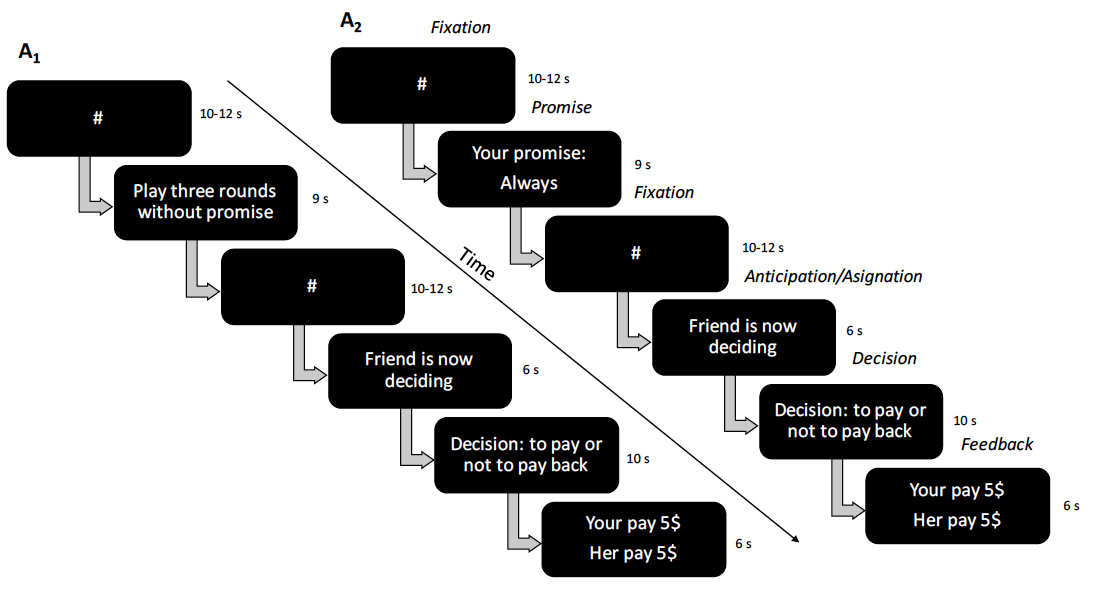
\includegraphics[width=0.8\linewidth]{/Users/saidjimenez/Documents/R/github_Said/social_closeness/Manuscript/figures/task} 

}

\caption{Trust game with promises, each box from left to right represents a screen that was shown to the subjects sequentially. Section A1 corresponds to an example of trials without promises and section A2 to trials with promises.}\label{fig:figA}
\end{figure}

Fixation phase consisted only of a period in which the subject paid
attention without performing any particular behavior. Then,
\textbf{promises phase} in part A1 indicated that in the following three
trials they could decide without the effect of the promise. In A2, the
subject was asked to decide between 1) always, 2) mostly, 3) sometimes
or 4) never pay back. This pattern was repeated. In the
\textbf{anticipation/assignation phase}, subjects were told who their
partner was for that trial (computer, stranger or friend) and was given
the message that their partner was making their decision. Later in the
\textbf{decision phase}, the subject was informed if his partner
invested his \$2 or not, he was reminded of his promise level (if they
were trails with promises) and, in case the partner had invested, he was
asked to decide whether to pay back or not. Finally, payments for each
trial were shown in the \textbf{feedback phase} and the sequence was
repeated until the task finished.

\hypertarget{procedure}{%
\subsection{Procedure}\label{procedure}}

Subjects came to the lab with a same-sex friend considered close by him
or her. It was emphasized that they must not have a romantic or family
relationship with their friends, to try to exclude the effect on
cooperation due to a consanguineous relationship or sexual attraction.
Also, to ensure that the subjects and their companions had a similar
degree of social closeness to each other, both responded the ``Inclusion
of the Other in Self'' IOS scale (Aron et al. 1997) without observing
their partner responses. The scale consists of seven pairs of circles
that vary in the degree of overlap between them, the respondent must
select the pair of circles that best represents the subjective closeness
to his partner. Subjects were trained in the main task by two
researchers, the game was first explained verbally, and then the
computer interface was presented on a portable computer. They were told
that they would make their decisions with four buttons on the computer
keyboard, which corresponded to the levels of promises and with only two
of these to make their decision to pay back or not. Friends heard the
explanation, they were told that they would make their decisions in a
separate room on another computer even though they were not. Subjects
performed between 3 and 6 practice tests together with the researcher
who exemplified the course of the game when the investor gave his
budget. When the subjects were ready, we proceeded to take them without
their companions to another room (or MRI scanner it that was the case)
where they would perform the task.The subjects began the task believing
that they would really play with the three partners of different social
closeness. In the other room, we debriefed the companion about the
deception. When the subject finished the task, they were debriefed.
Although no participant exercised their right, both subjects and their
friends were told that they could withdraw their participation and
informed consent if they considered disagreeing with any of the
manipulations made by the researchers.

\hypertarget{bayesian-modeling}{%
\subsection{Bayesian Modeling}\label{bayesian-modeling}}

All models presented below were programmed in R via the \textbf{brms}
package (Bürkner 2017; R Core Team 2019), which performs the inference
using sampling by Markov chain Monte Carlo through \textbf{Stan} (Stan
Development Team 2018). For each model, the posteriors distributions of
all parameters were approximated with four chains of 2000 iterations
each, the first 1000 iterations of each chain were discarded (burning
period), for a total of 4000 post burning samples. Models convergence
was evaluated through visual inspection of the chains and calculation of
the \(\hat{R}\) statistic, which for all parameters was 1, that can be
interpreted as convergence. Vaguely informative prior distributions were
used for the parameters of interest in the models, which allows the data
to dominate the inference, also assumes as little as possible regarding
the nature of the phenomenon, which could be adequate for the current
state of evidence in the problem we are studying (McElreath 2018).

\hypertarget{results}{%
\section{Results}\label{results}}

\hypertarget{descriptives}{%
\subsection{Descriptives}\label{descriptives}}

We analyzed 810 decisions about paying back or not (18 per subject), as
well as 180 promises (4 per subject). 69\% of the decisions, were pay
back, while the proportion of the promises selected were never = 5.4\%,
sometimes = 16.2\%, mostly = 43.8\% and always = 40.2\%. Figure 2 shows
the payment proportion depending on the levels of promises and partners.
Breaking promises, meaning the subject had promised always and
subsequently decides not to pay back, occurred only in 12.4\% of trials
(19 times they did not pay back of 153 when promised always), of which,
8.50\% (13/153) were trials with the computer, 3.92\% (6/153) with the
stranger and 0\% (0/153) with the friend. It is essential to note that
breaking the promise was not the most frequent decision, when they
promised always and had the computer as a partner, they decided to pay
back in 91.5\% of trials.

\begin{figure}

{\centering 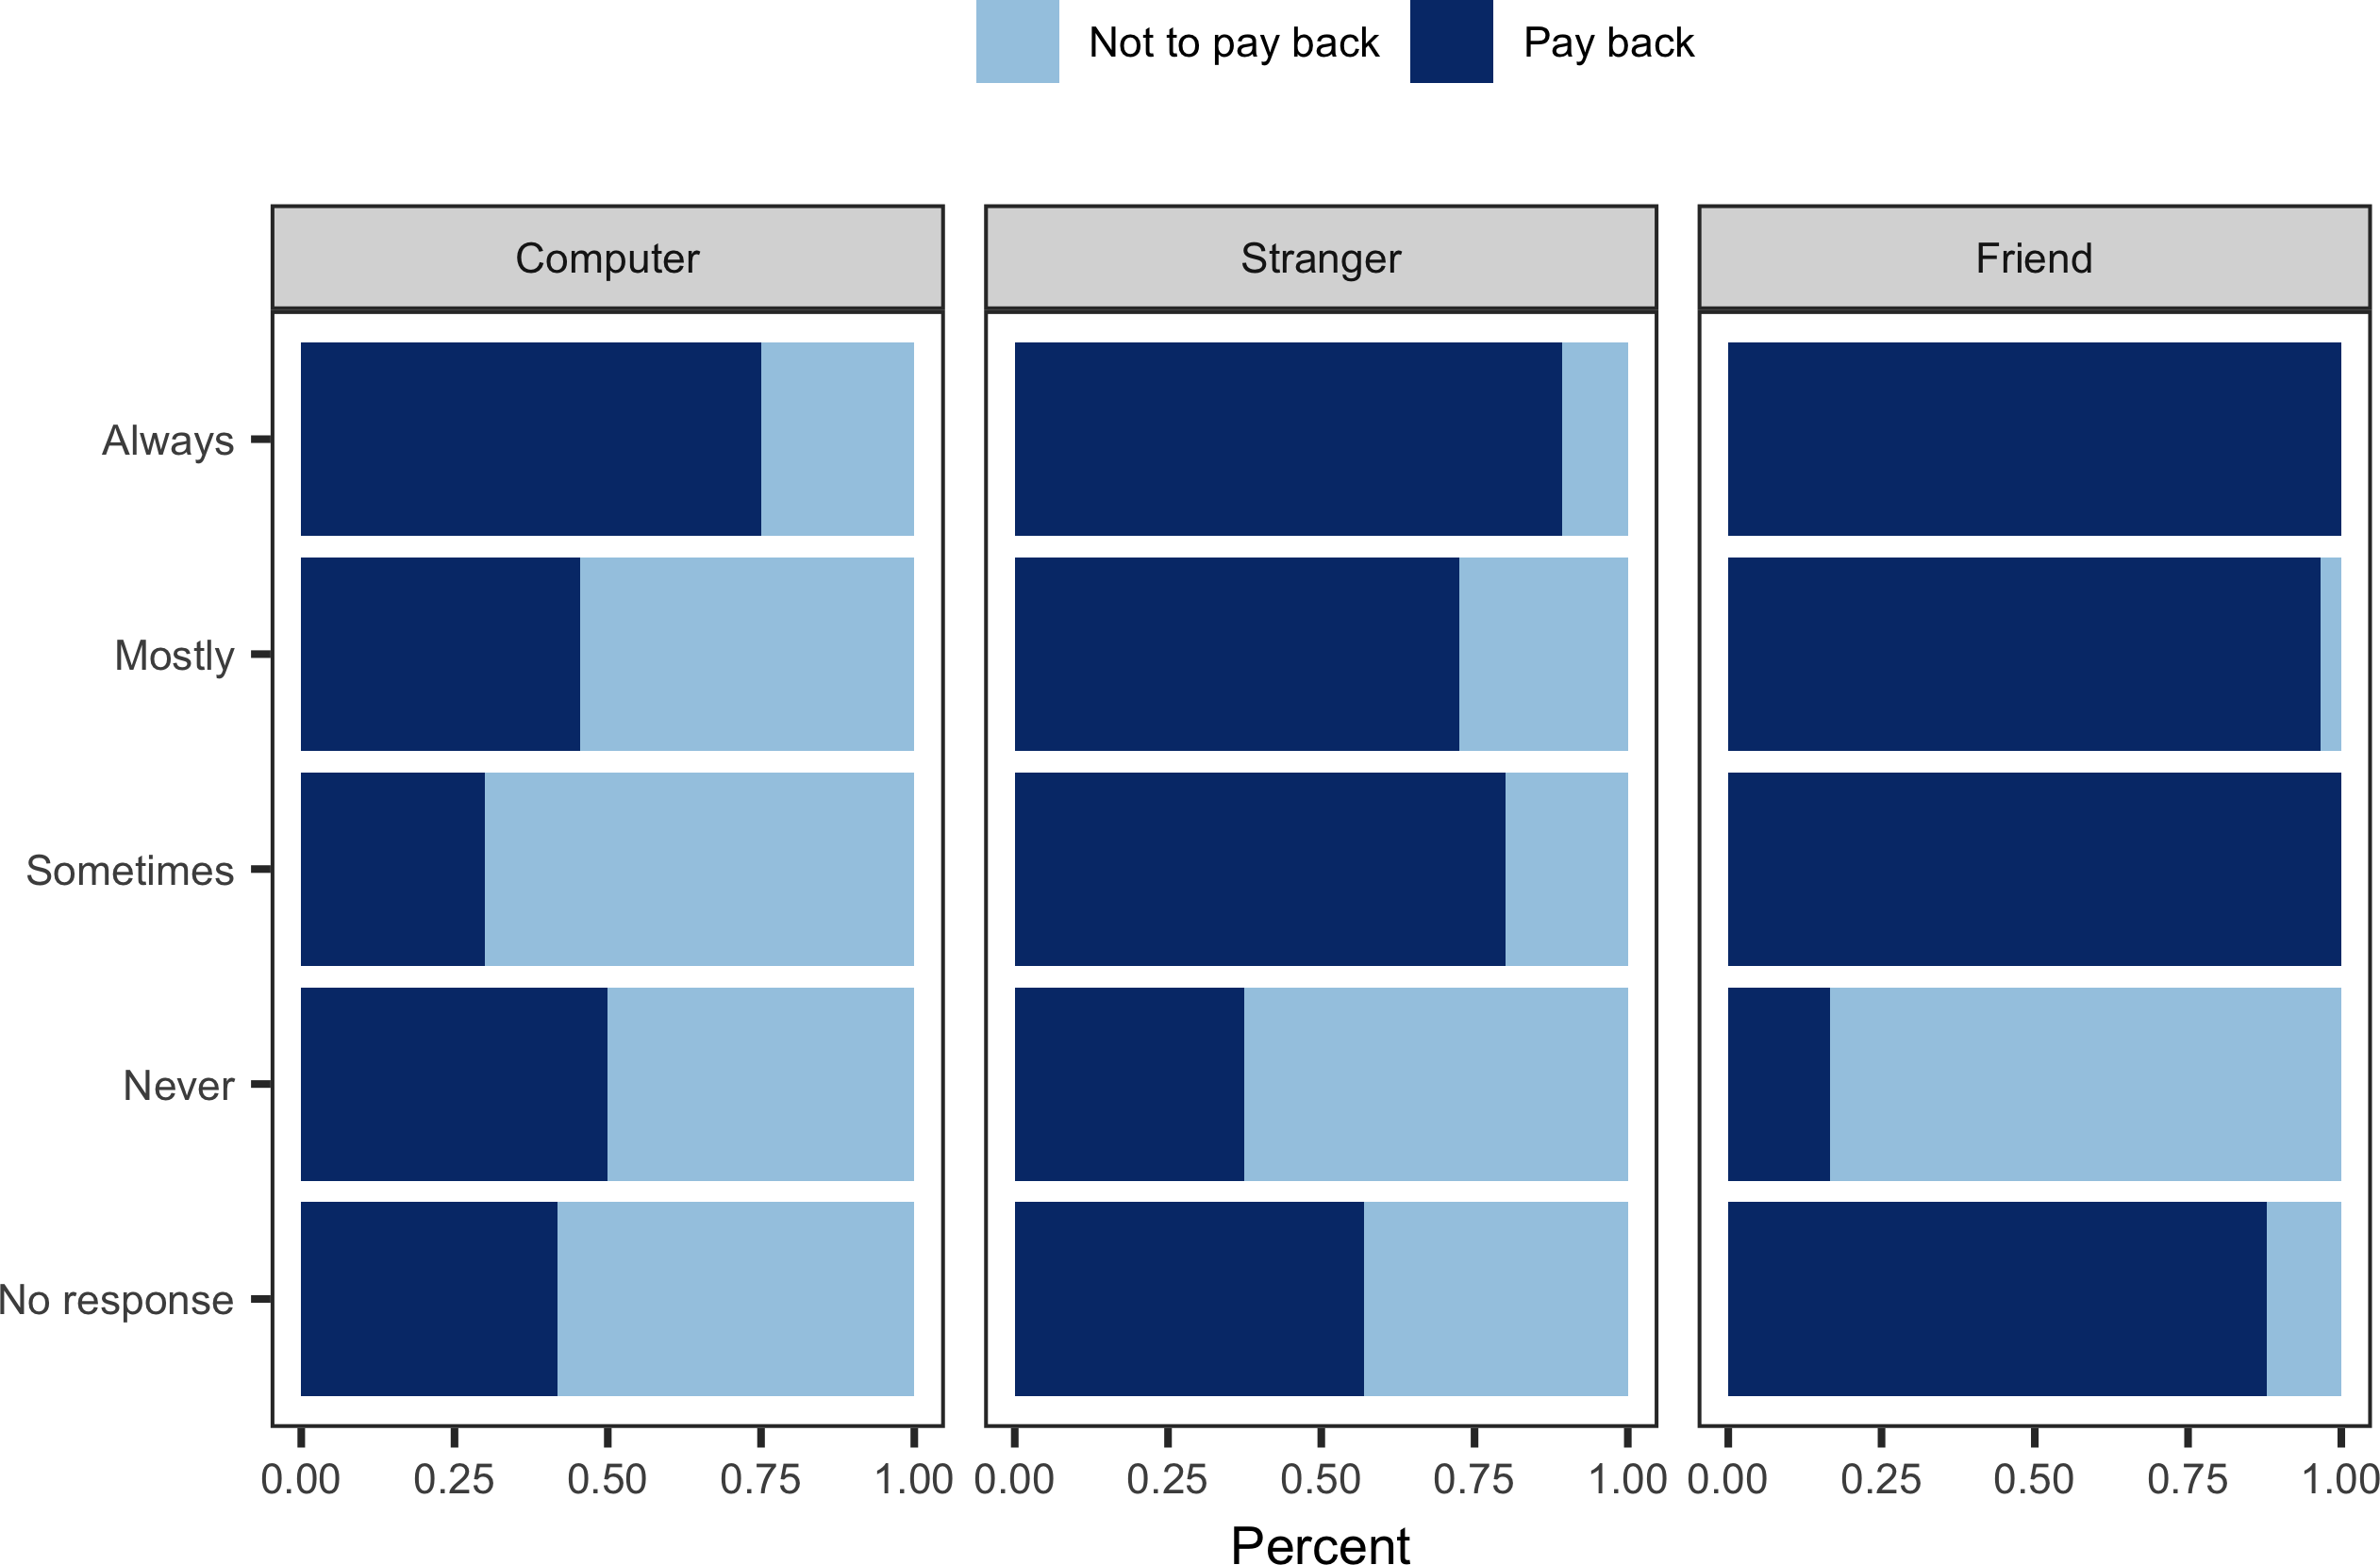
\includegraphics[width=0.8\linewidth]{behavioral-promises_files/figure-latex/fig2-1} 

}

\caption{Pay back proportion by partners and promises levels}\label{fig:fig2}
\end{figure}

\hypertarget{social-closeness-between-partners}{%
\subsubsection{Social closeness between
partners}\label{social-closeness-between-partners}}

To assess social closeness, 30 (15 men) of our subjects and their
friends responded to the IOS scale (Aron et al. 1997; Fareri and Delgado
2014; Sip et al. 2015), which consists of seven pairs of circles that
vary in the degree of overlap and represent the social closeness that an
individual perceives with respect to the other. A Hierarchical and
Cumulative Bayesian Model (See section: Commitment expressed in the
promises), supports the hypothesis that there are no differences in
subjective social closeness between subjects and their friends, with a
posterior evidence ratio of 2.74 in its favor.

\hypertarget{hierarchical-bayesian-modeling}{%
\subsection{Hierarchical Bayesian
Modeling}\label{hierarchical-bayesian-modeling}}

\hypertarget{effect-of-social-closeness-on-breaking-promises}{%
\subsubsection{Effect of social closeness on breaking
promises}\label{effect-of-social-closeness-on-breaking-promises}}

To evaluate the hypothesis that social closeness would reduce the
behavior of breaking the promise, we filtered all trials in which
subjects promised that they would always pay back and then decided not
to pay. Subsequently, Bayesian inference was used to assess the effect
of partners on the decision to break the promise at the individual and
population level. For this purpose, a Hierarchical Bayesian Model was
carried out that assumes that the uncertainty in partners effect on the
decision to break the promise varies depending on each individual,
however, it also assumes that these variations belong to common
population distributions (Gelman and Hill 2006).

\[
\begin{aligned}
&y_i \sim \mathrm{Bernoulli}(\theta_i) \\
&\mathrm{logit(\theta_i)} = \mathbf{X}\beta  +  \mathbf{Z}u
\end{aligned}
\]

In the previous model, the decision to break the promise \(y_i\) comes
from a Bernoulli distribution with probability \(\theta_i\), the goal of
the Hierarchical Model is to predict each decision through the linear
combination of the effects of each partner, transformed by its inverse
link function \(\mathrm{logit}\) (Bürkner 2017). In this model,
\(\beta\) and \(u\) are coefficients at the population level and
individual level respectively, while \(\mathbf{X}\), \(\mathbf{Z}\) are
their corresponding design matrices. In this case, the population
coefficients correspond to the presence of partners with no social
closeness \(\beta^{computer}\), low \(\beta^{stranger}\) and high
\(\beta^{friend}\).

Figure 3 shows the posterior probability of breaking the promise
depending on the partner, circles correspond to the medians of the
distributions of the posterior estimates effects, the thick bar, and the
thin bar correspond to the interval of 50\% and 95\% posterior
probability, respectively. It is clear that the probability of breaking
the promise decreases as social closeness increases, however, we
calculate the reasons for evidence for the following hypotheses:

\begin{itemize}
\item
  There is a greater probability to break the promise to the computer
  than the stranger.
\item
  There is more probability to break the promise to the stranger
  compared to a friend.
\end{itemize}

The evidence ratio, which is the ratio between the posterior probability
of the mentioned hypotheses and their corresponding alternative
hypotheses was 7.47 and 8.64 respectively in favor of the previous
hypotheses. As seen in Figure 5 in the estimate for
\(\beta^{computer}\), no social closeness, we have a 95\% posterior
probability that the parameter for promise-breaking is between 4-38\%,
although it is a small proportion, it clearly excludes the probability
that promises are not broken.

\begin{figure}

{\centering 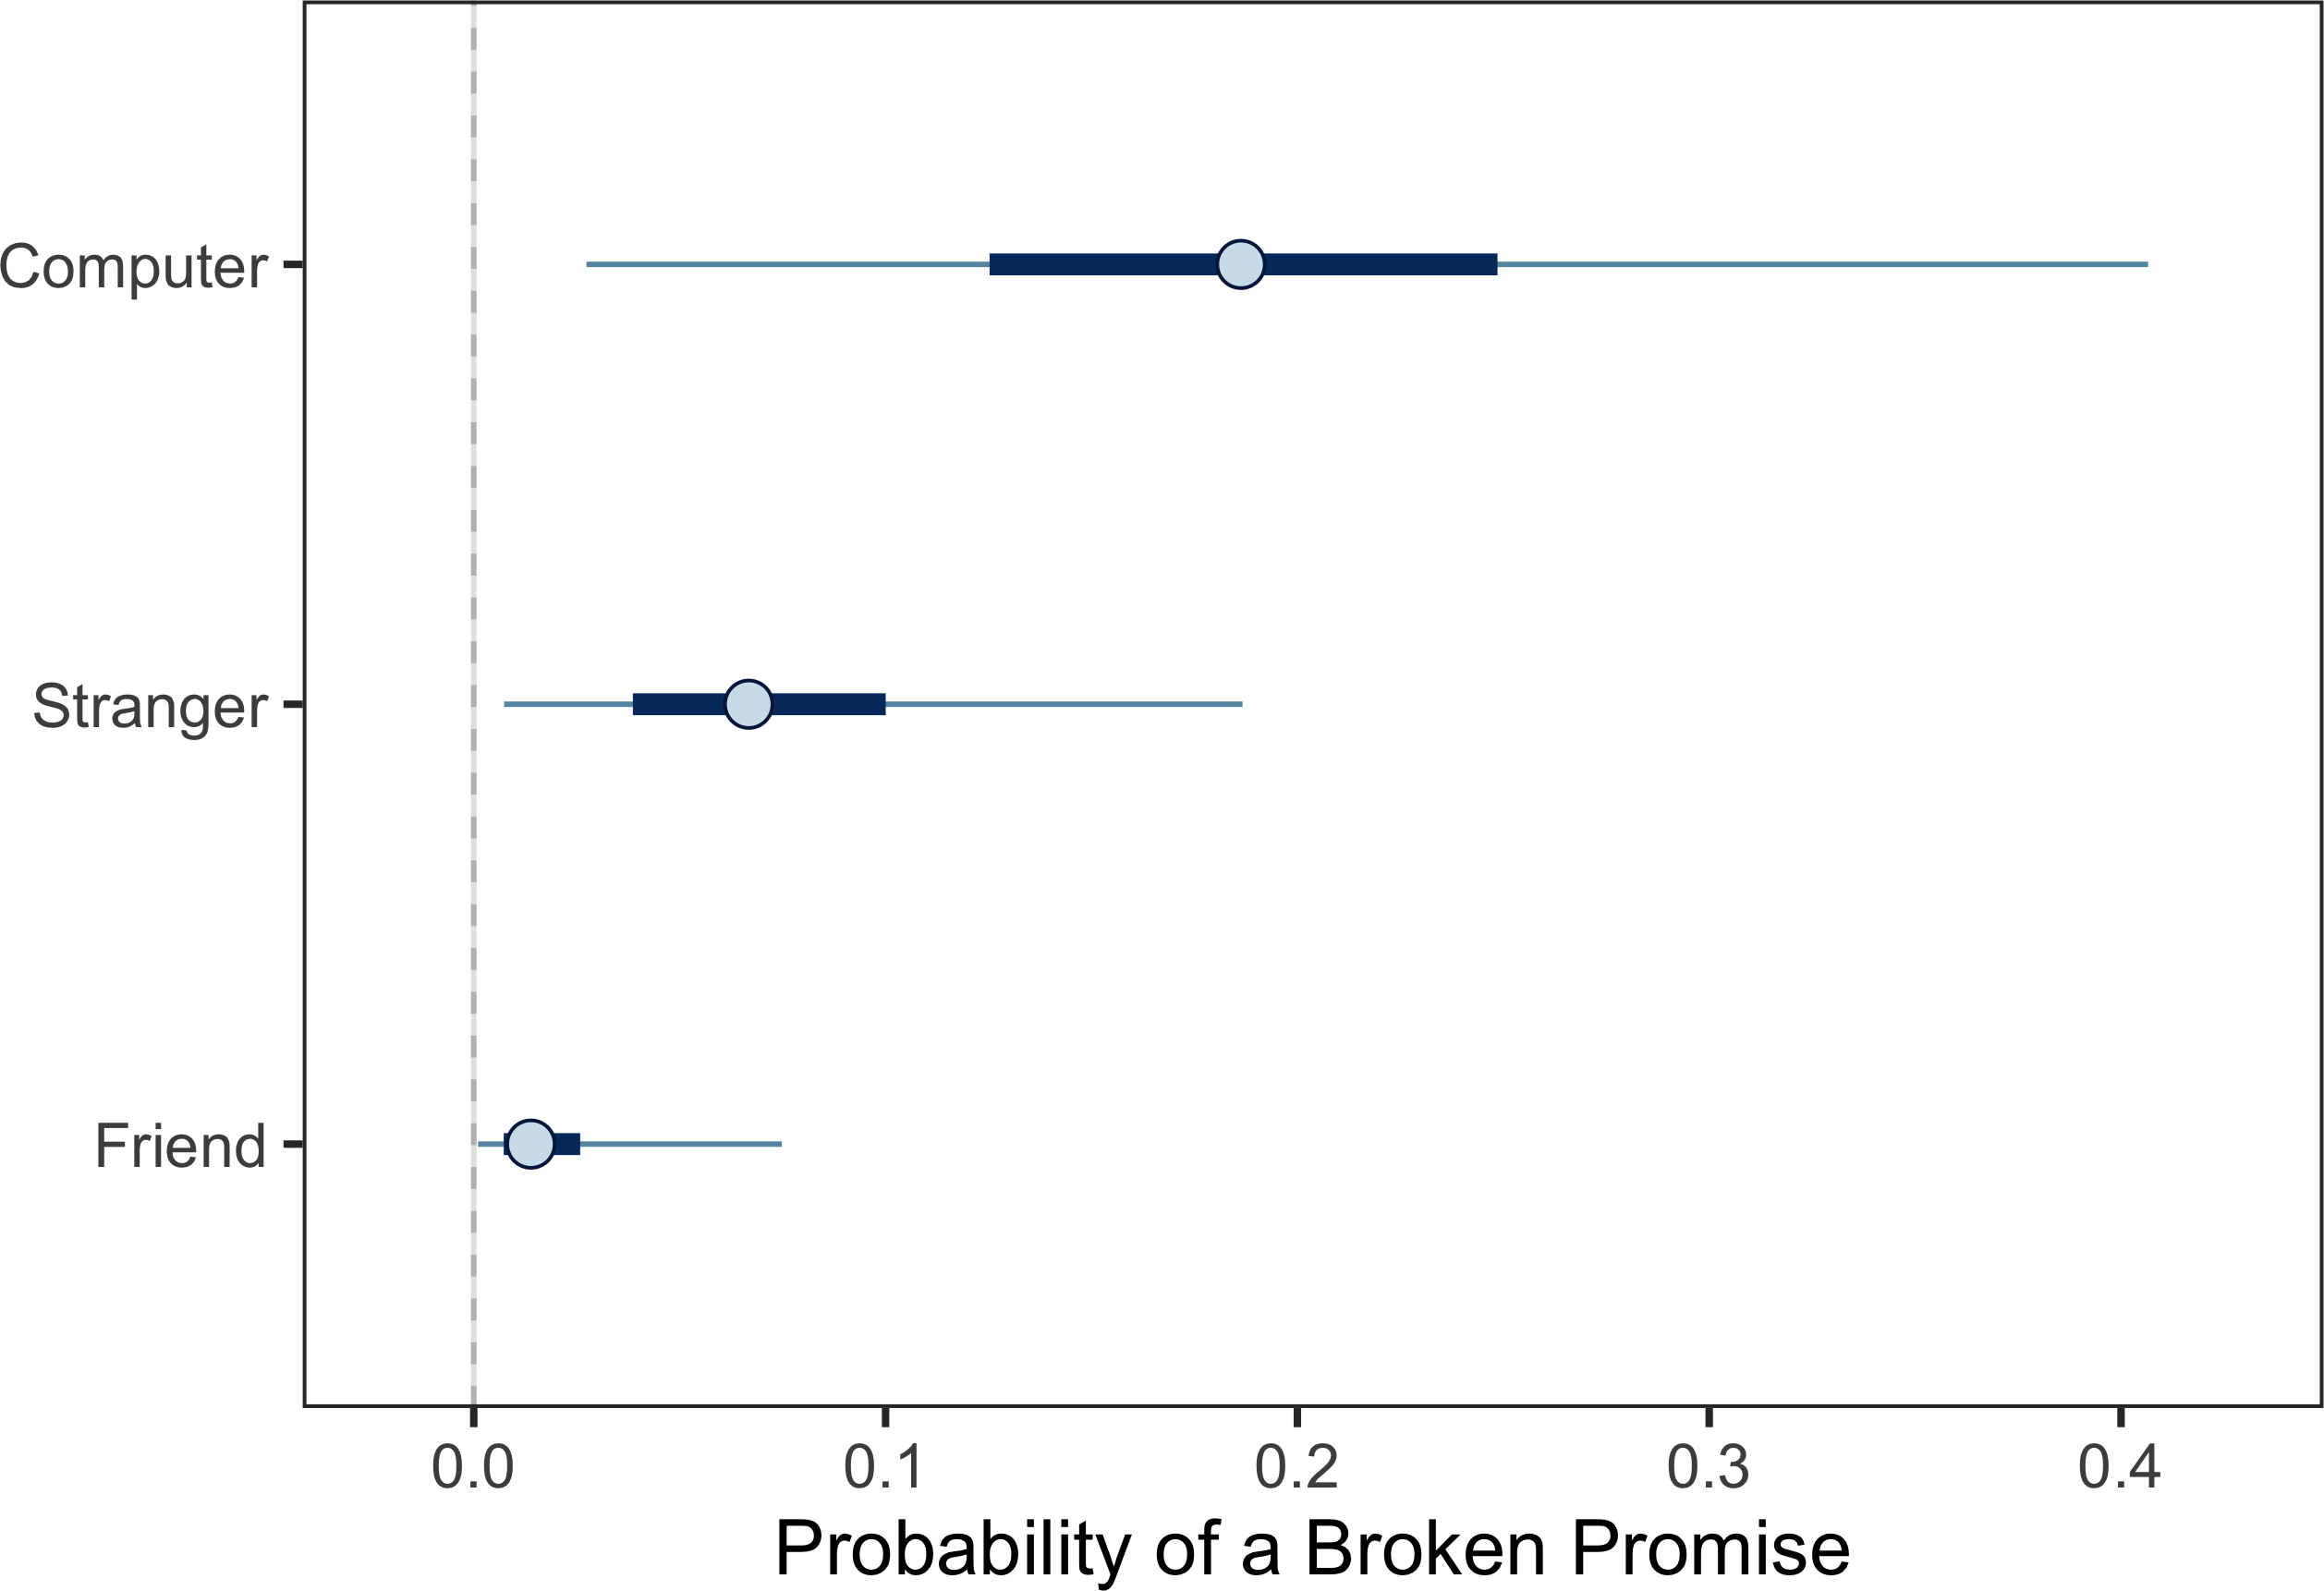
\includegraphics[width=0.8\linewidth]{behavioral-promises_files/figure-latex/fig3-1} 

}

\caption{Posterior probability of Promise Breaking}\label{fig:fig3}
\end{figure}

\hypertarget{effects-of-promises-and-social-closeness-on-cooperation}{%
\subsubsection{Effects of promises and social closeness on
cooperation}\label{effects-of-promises-and-social-closeness-on-cooperation}}

To evaluate the effect of the experimental conditions on the decision to
pay back, we used all trials were partners invest. Again, a Hierarchical
Bayesian Model was fit, which assumes that the promises and partners
have an effect that varies for each individual, however, it also assumes
that these variations belong to common population distributions. The
model estimates that the probability \(\theta_i\) of the decision to pay
back is based on the effect of the presence of promises
\(\beta^{promise}\), as well as partners with low \(\beta^{stranger}\)
and high \(\beta^{friend}\) social closeness.

Figure 4 shows the posterior distributions of the \(\beta\) coefficients
in the logit scale, the center line represents the median of the
distribution and the shaded area corresponds to the interval of 50\%
posterior probability. As shown, more than 95\% of the posterior density
of the population coefficients is greater than 0, which shows strong
evidence of the effect of experimental conditions on the decision to pay
back, although the presence of promises and the stranger clearly
increase the probability of paying, the presence of the friend is the
condition that has the greatest effect on this behavior. Posterior
distributions clearly show that the probability of cooperation increases
as social closeness does.

\begin{figure}

{\centering 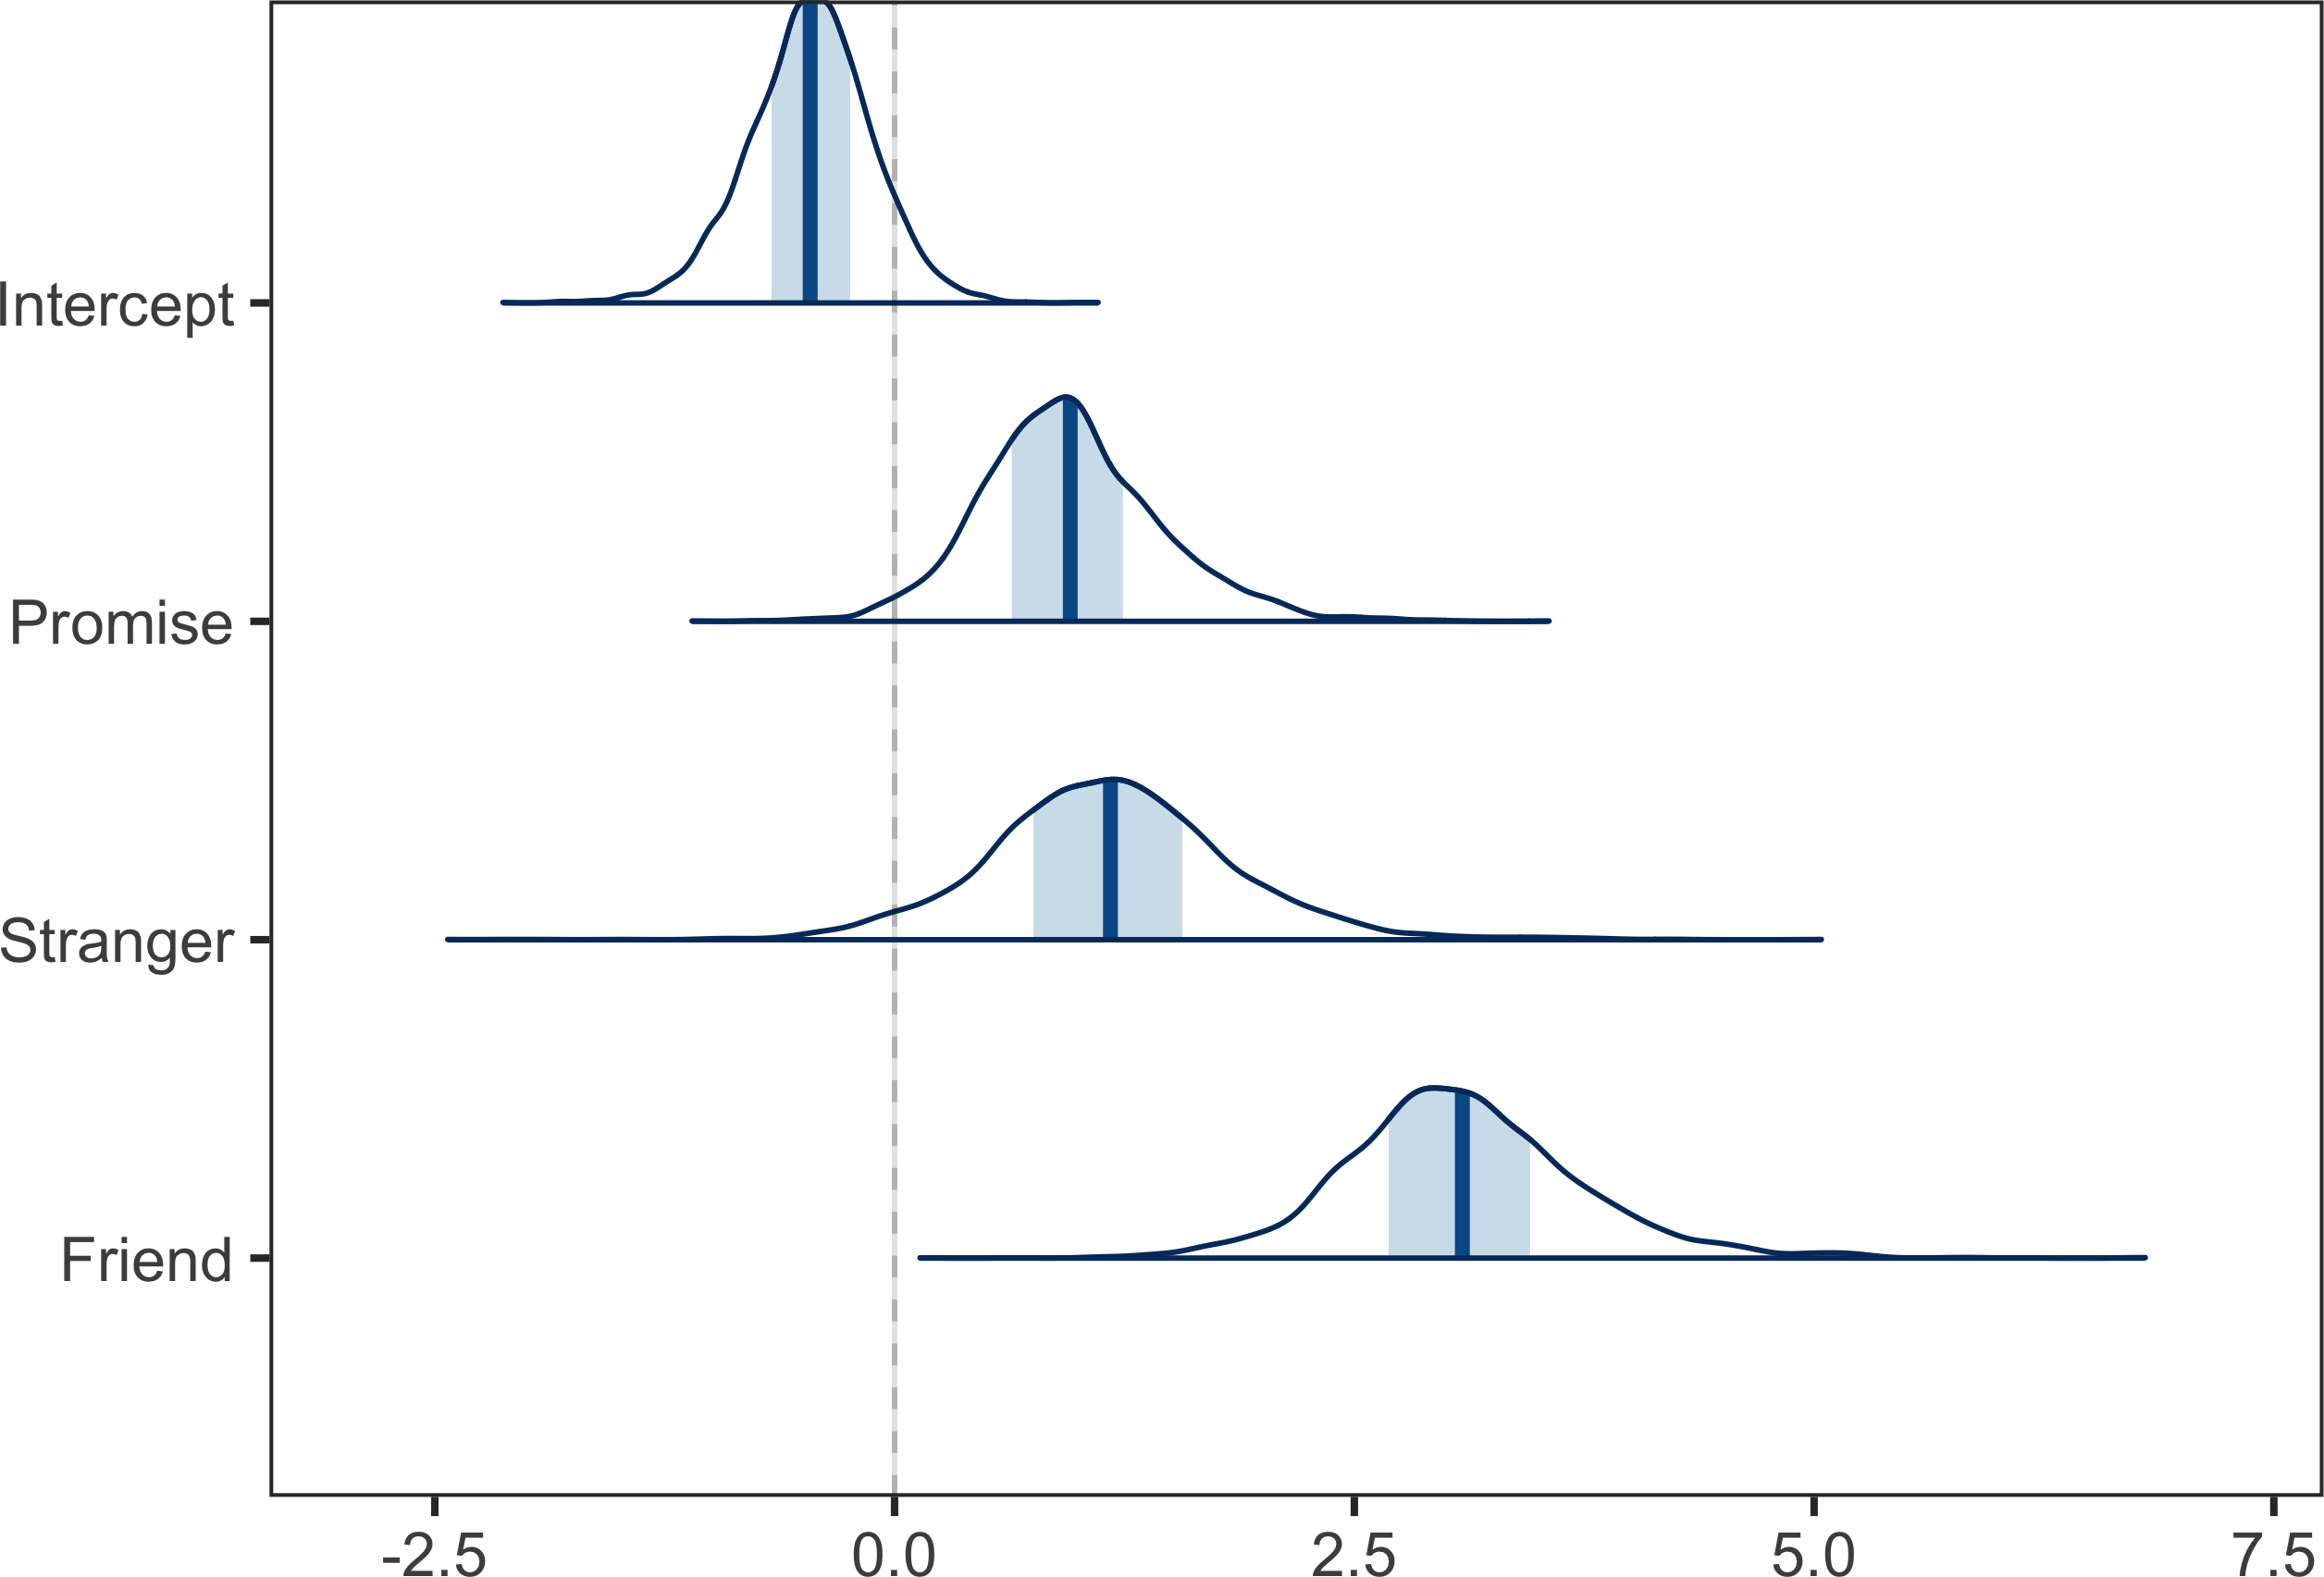
\includegraphics[width=0.8\linewidth]{behavioral-promises_files/figure-latex/fig4-1} 

}

\caption{Posterior estimates in logit scale}\label{fig:fig4}
\end{figure}

Figure 5 shows the posterior predictive distribution in contrast to the
proportion of decisions to each partner during the promises phase, and
each panel corresponds to one of the first twelve subjects. The
responses on the dotted line would indicate that the subject paid back
random to that partner. Posterior predictive distribution simulates
observations of the model and compares them with the actual data, it
helps us to identify if the model is sufficiently close to the process
that generated the data (Schad, Betancourt, and Vasishth 2019; Lee and
Wagenmakers 2014). It can be seen that there is a great correspondence
between the subject's responses and predictions of the model. Even in
cases where the model is ``wrong'' (for example, subject 1), the
observed response is in the range of a predicted standard deviation,
which gives credibility to estimates.

\begin{figure}

{\centering 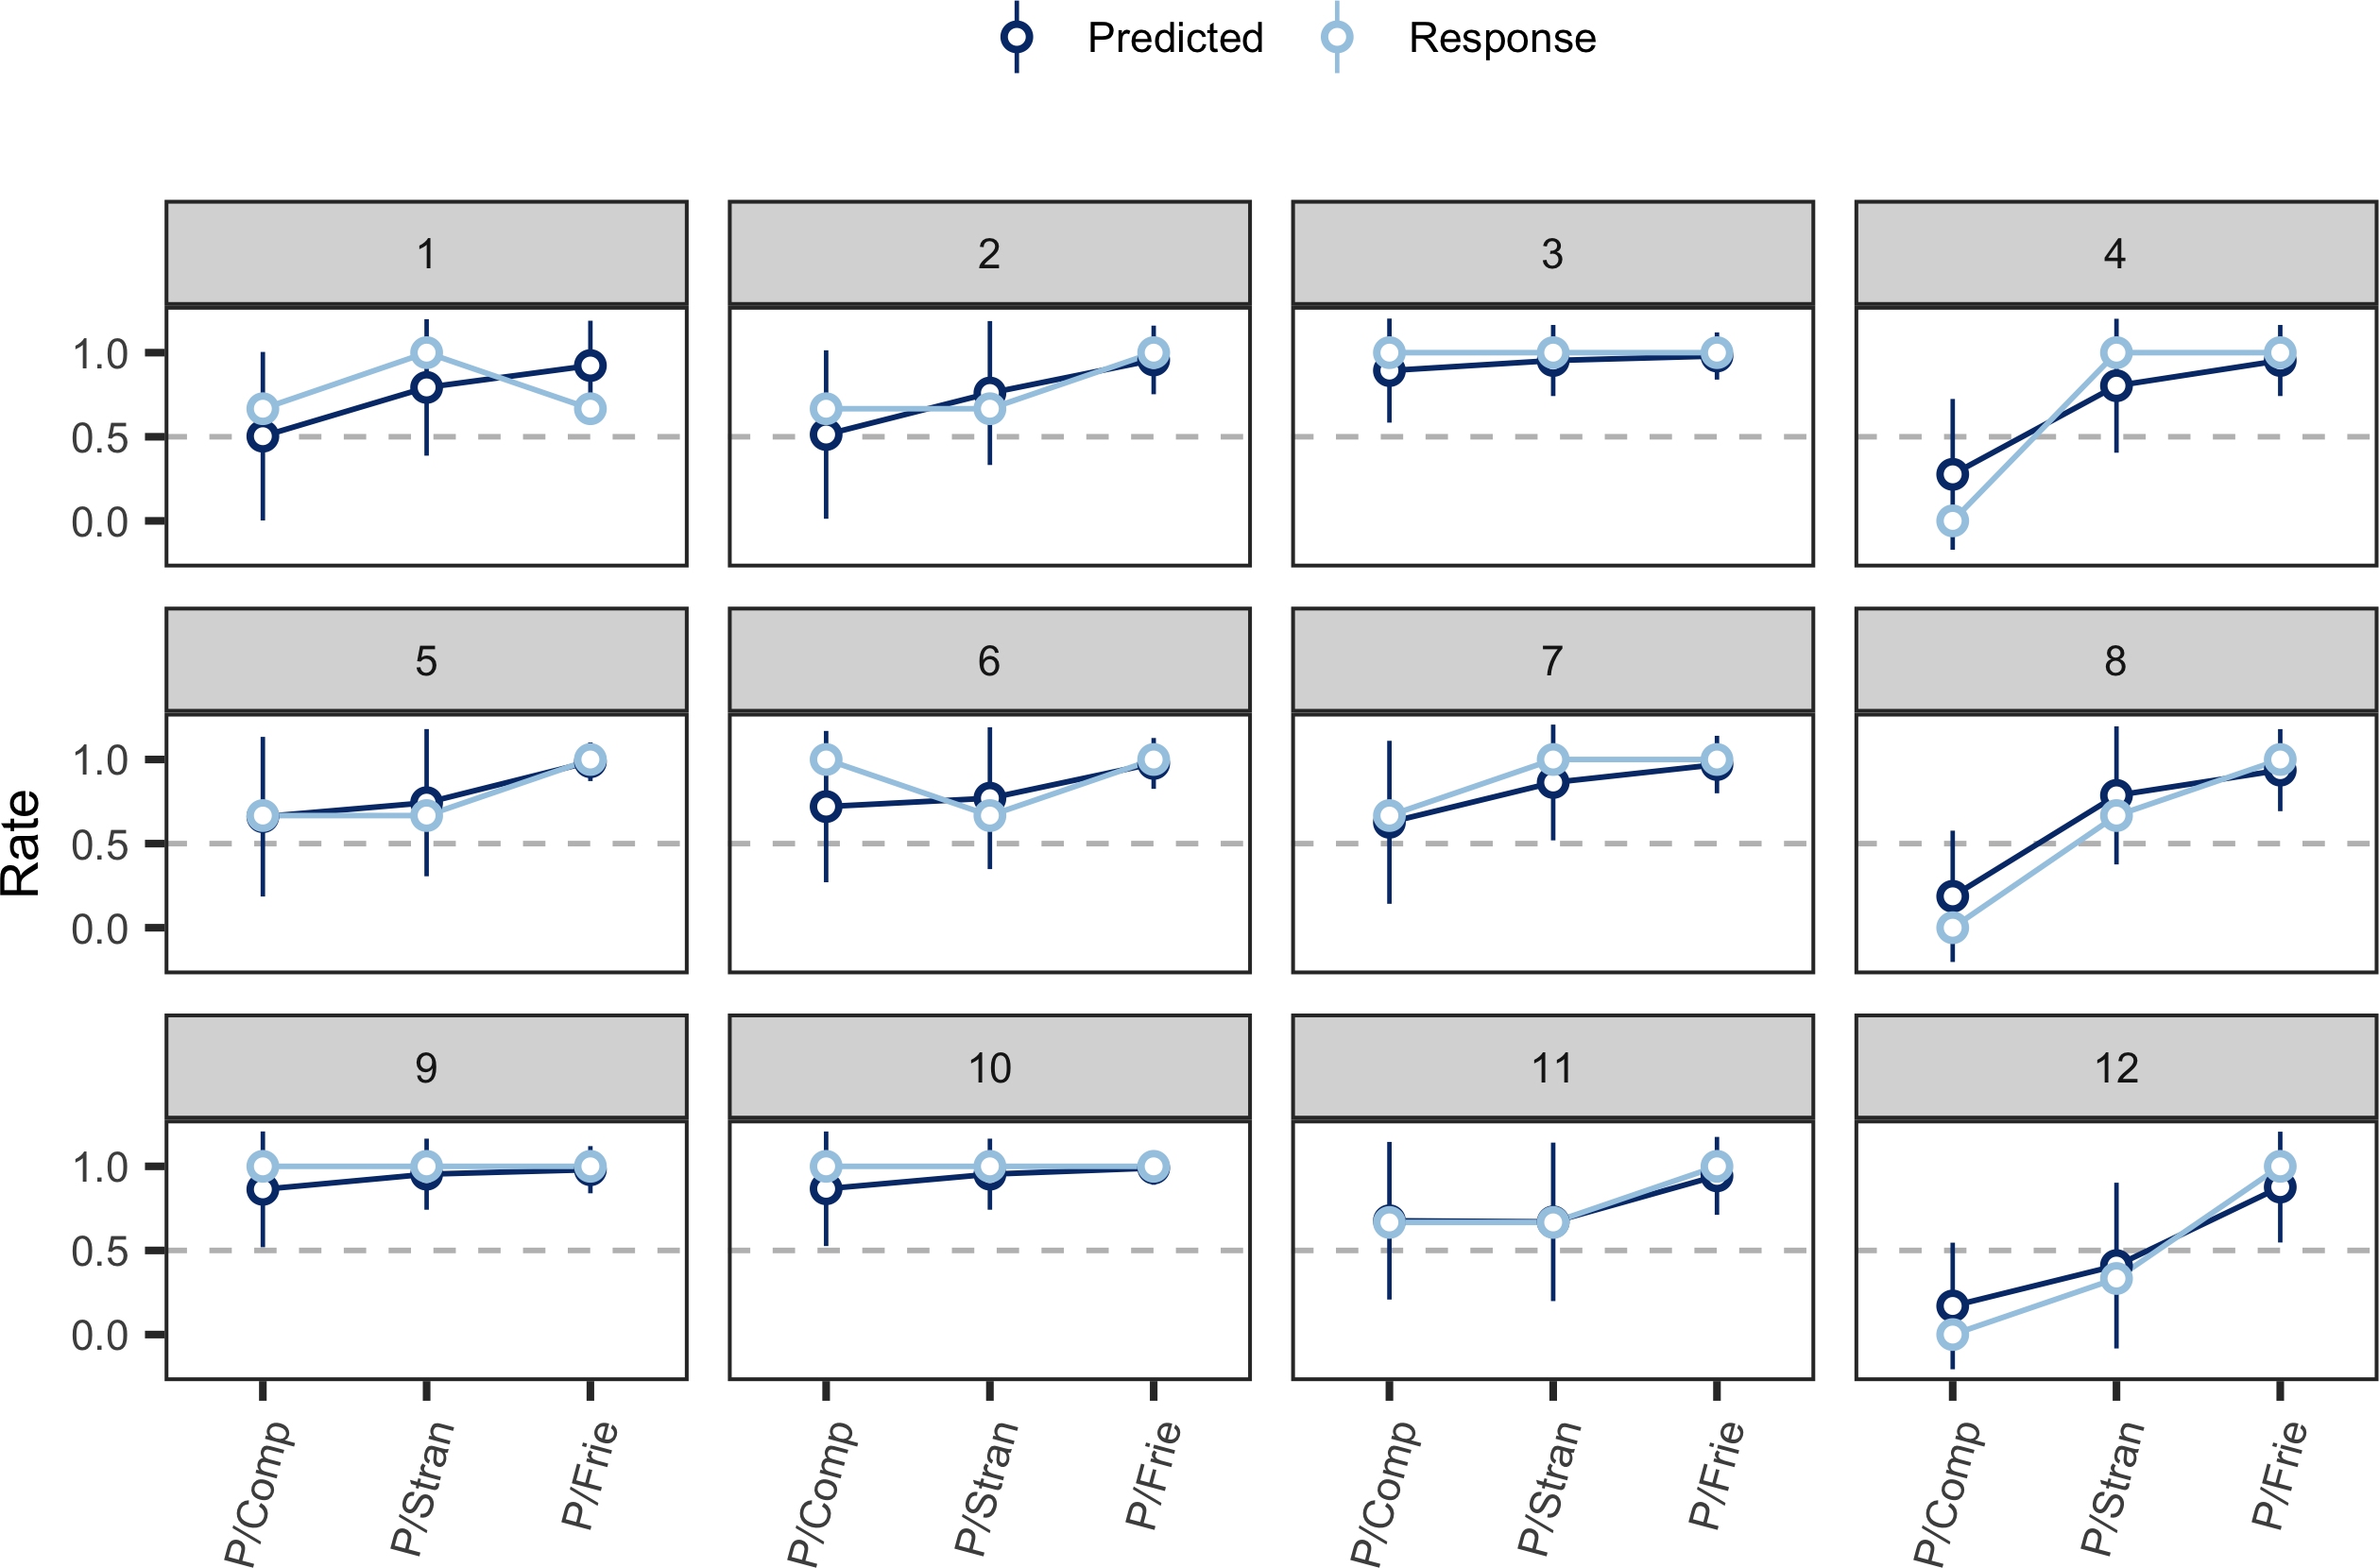
\includegraphics[width=1\linewidth,height=0.42\textheight]{behavioral-promises_files/figure-latex/fig5-1} 

}

\caption{Posterior predictive over pay back rate}\label{fig:fig5}
\end{figure}

\hypertarget{effects-of-social-closeness-on-cooperation-varying-by-promises}{%
\subsubsection{Effects of social closeness on cooperation varying by
promises}\label{effects-of-social-closeness-on-cooperation-varying-by-promises}}

In this model, it is assumed that social closeness has an effect that
varies for each level of promise, which implies that there are levels of
promise that are more sensitive than others to the effect of the
partner's on the decision to pay back. Again, a Hierarchical Bayesian
Model was made to estimate the effect of partners at the population
level and the variations depending on the promise levels. Table 1
summarizes the subsequent distributions of the model coefficients in the
logit scale, including point estimates, standard errors and Bayesian
Credibility Intervals of 95\%. An estimate similar to the previous
models can be observed, with strong evidence of the effect of social
closeness on the decision to pay back. Although the credibility range
for the friend's effect includes 0, the evidence ratio that the effect
is greater than zero is 15.81 with 94\% of posterior probability.

\begin{figure}

{\centering 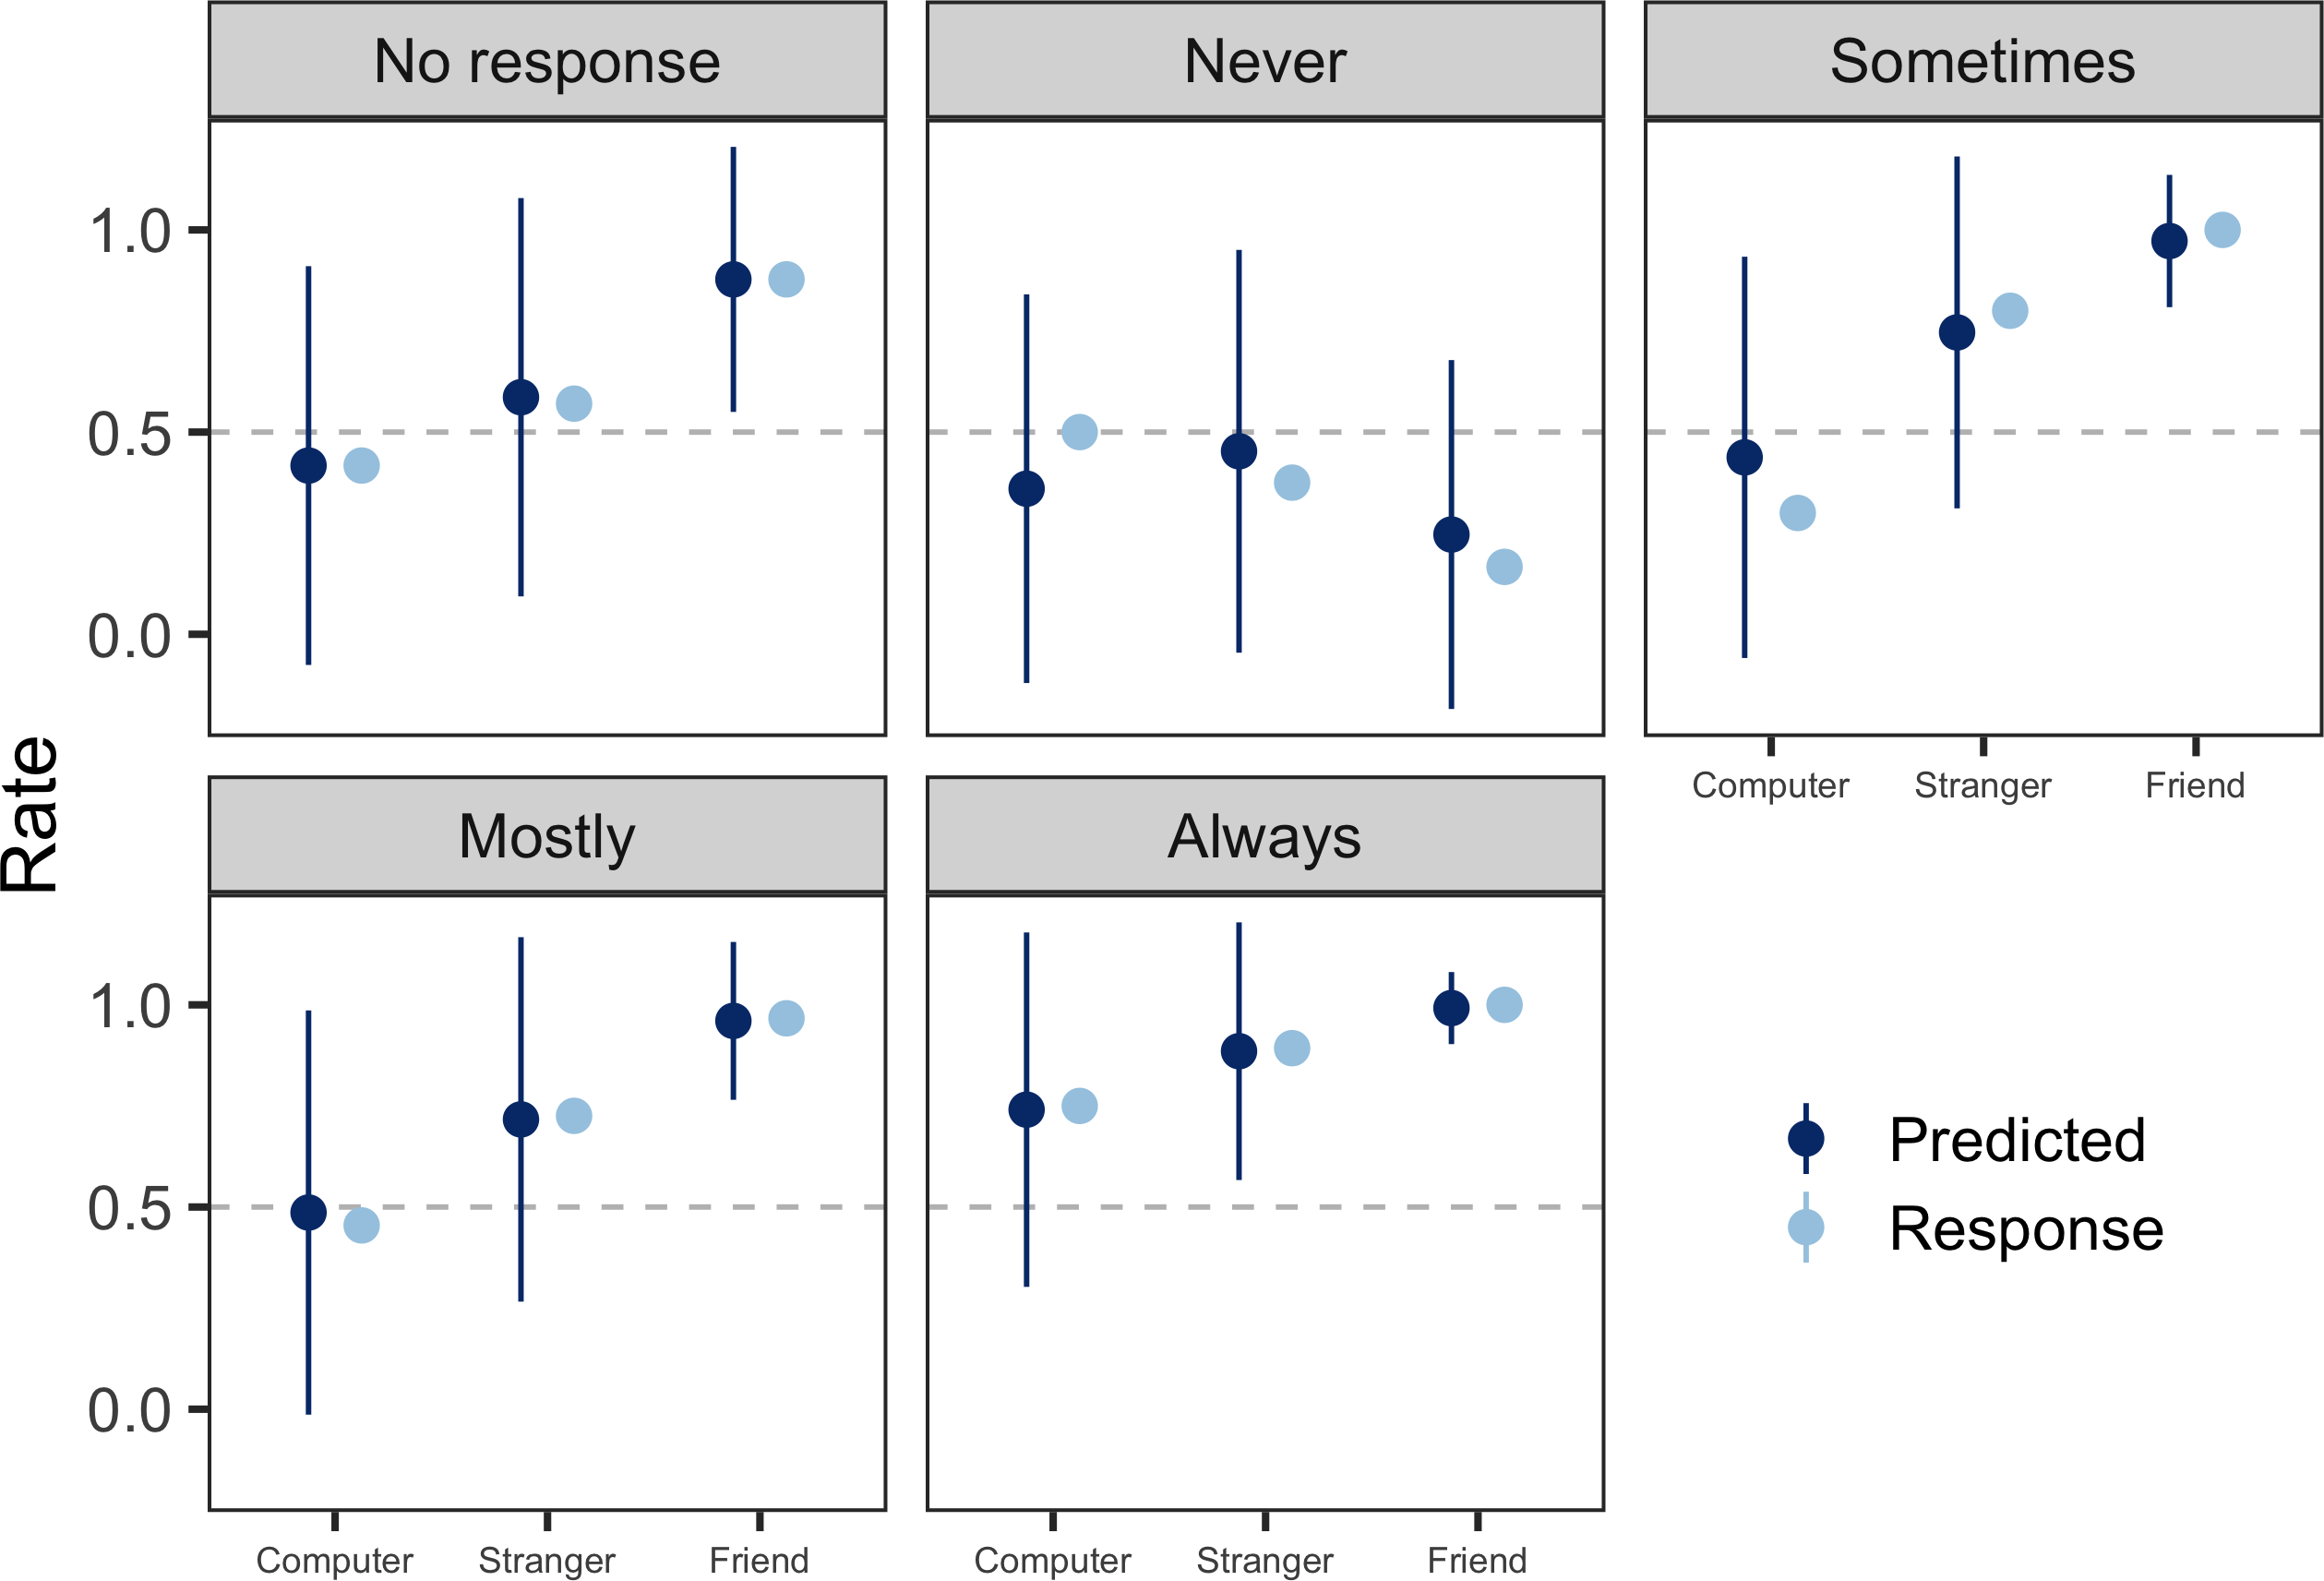
\includegraphics[width=0.8\linewidth]{behavioral-promises_files/figure-latex/fig6-1} 

}

\caption{Posterior predictive over pay back rate, Social Closeness Varying effects by Promise levels}\label{fig:fig6}
\end{figure}

On the other hand, Figure 6 shows the posterior predictive distribution,
compared to the payment rates of all individuals to the different
partners and their variation by the level of promise. With the exception
of the promise never, a monotonic positive effect of partners is
observed at all levels of promise. However, we also observe how the
effect of social closeness varies depending on the strength of the
promise, mainly for the decisions towards the computer.

\begin{table}[t]

\caption{\label{tab:tabla}Posterior coefficients estimates}
\begin{tabular}{lrrrr}
\toprule
\multicolumn{1}{c}{ } & \multicolumn{2}{c}{ } & \multicolumn{2}{c}{95 \% CI} \\
\cmidrule(l{3pt}r{3pt}){4-5}
Term & Estimate & Est.Error & Lower & Upper\\
\midrule
Intercept & -0.153 & 0.536 & -1.005 & 0.617\\
Stranger & 0.829 & 0.410 & 0.128 & 1.470\\
Friend & 2.084 & 1.248 & -0.151 & 3.975\\
\bottomrule
\end{tabular}
\end{table}

\hypertarget{cumulative-bayesian-modeling}{%
\subsection{Cumulative Bayesian
Modeling}\label{cumulative-bayesian-modeling}}

\hypertarget{commitment-expressed-in-promises}{%
\subsubsection{Commitment expressed in
promises}\label{commitment-expressed-in-promises}}

In the original study of promises, authors chose to divide their sample
into two according to the hierarchical clustering technique with Ward's
method (Baumgartner et al. 2009). In this way they obtained two sets of
participants that were different in their payment rates, despite the
fact that they both made very high promises. For this reason, the
authors named the group that paid little as ``dishonest'' and the group
that paid a lot as ``honest''. In a similar exercise, in the present
study we performed the hierarchical grouping technique to obtain a
solution for two groups and we found two similar sets in n that we call
the group ``Low'' and ``High'' (Low = 25, High = 20), with quite
different payment ratios (Low = 58\%, High = 83\%), and a 95\%
confidence interval of 20\% to 32\% in the difference favor of the High
group.

Although it seems a similar result to that reported in that paper
(Baumgartner et al. 2009), we explore the pattern of promises of both
groups to determine if it was possible to classify our subjects as
honest and dishonest. If we hypothesize that the commitment to pay would
be reflected in the level of promises selected, a group of dishonest
people could generate in their partners the belief that they will pay by
choosing a high level of promises (mostly or always) and, later,
betraying that trust when deciding not to pay back. In order to explore
whether the groups represent populations that do not differ in the level
of commitment expressed in the promises, we use a Cumulative Bayesian
Model, which assumes that the levels of promises are an observed ordinal
variable \(Y\) that originates from the categorization of a continuous
latent variable \(\tilde{Y}\), for this case, the expressed commitment
to pay back (Bürkner and Vuorre 2019). The degree to which the subjects
of the High group differ from the Low group, in normal standard
deviations (\(z\)-values), on the latent scale of \(\tilde{Y}\), has a
point estimate of 0.95, which implies that the High group has 0.95
z-values greater commitment to pay back than the Low group. The 95\%
Bayesian Credibility Interval indicates that the High group is between
0.40 to 1.51 \(z\)-values of difference from Low. So we can conclude
with at least a 95\% probability that people belonging to the High group
expressed in their promises a greater commitment to pay back than the
subjects of the Low group. If we look at Figure 7, the probability of
choosing the different levels of promises varies depending on the group,
the one who had the highest percentage of decisions to pay back is more
likely to choose always (High group), while the group that had the
lowest percentage of decisions to pay back are more likely to choose
mostly (Low group). According to our data, we could not justify the
classification of our groups according to their honesty or dishonesty,
at least not with the technique used in Baumgartner et al. (2009). Since
people were quite consistent with keeping what they promised to pay.

\begin{figure}

{\centering 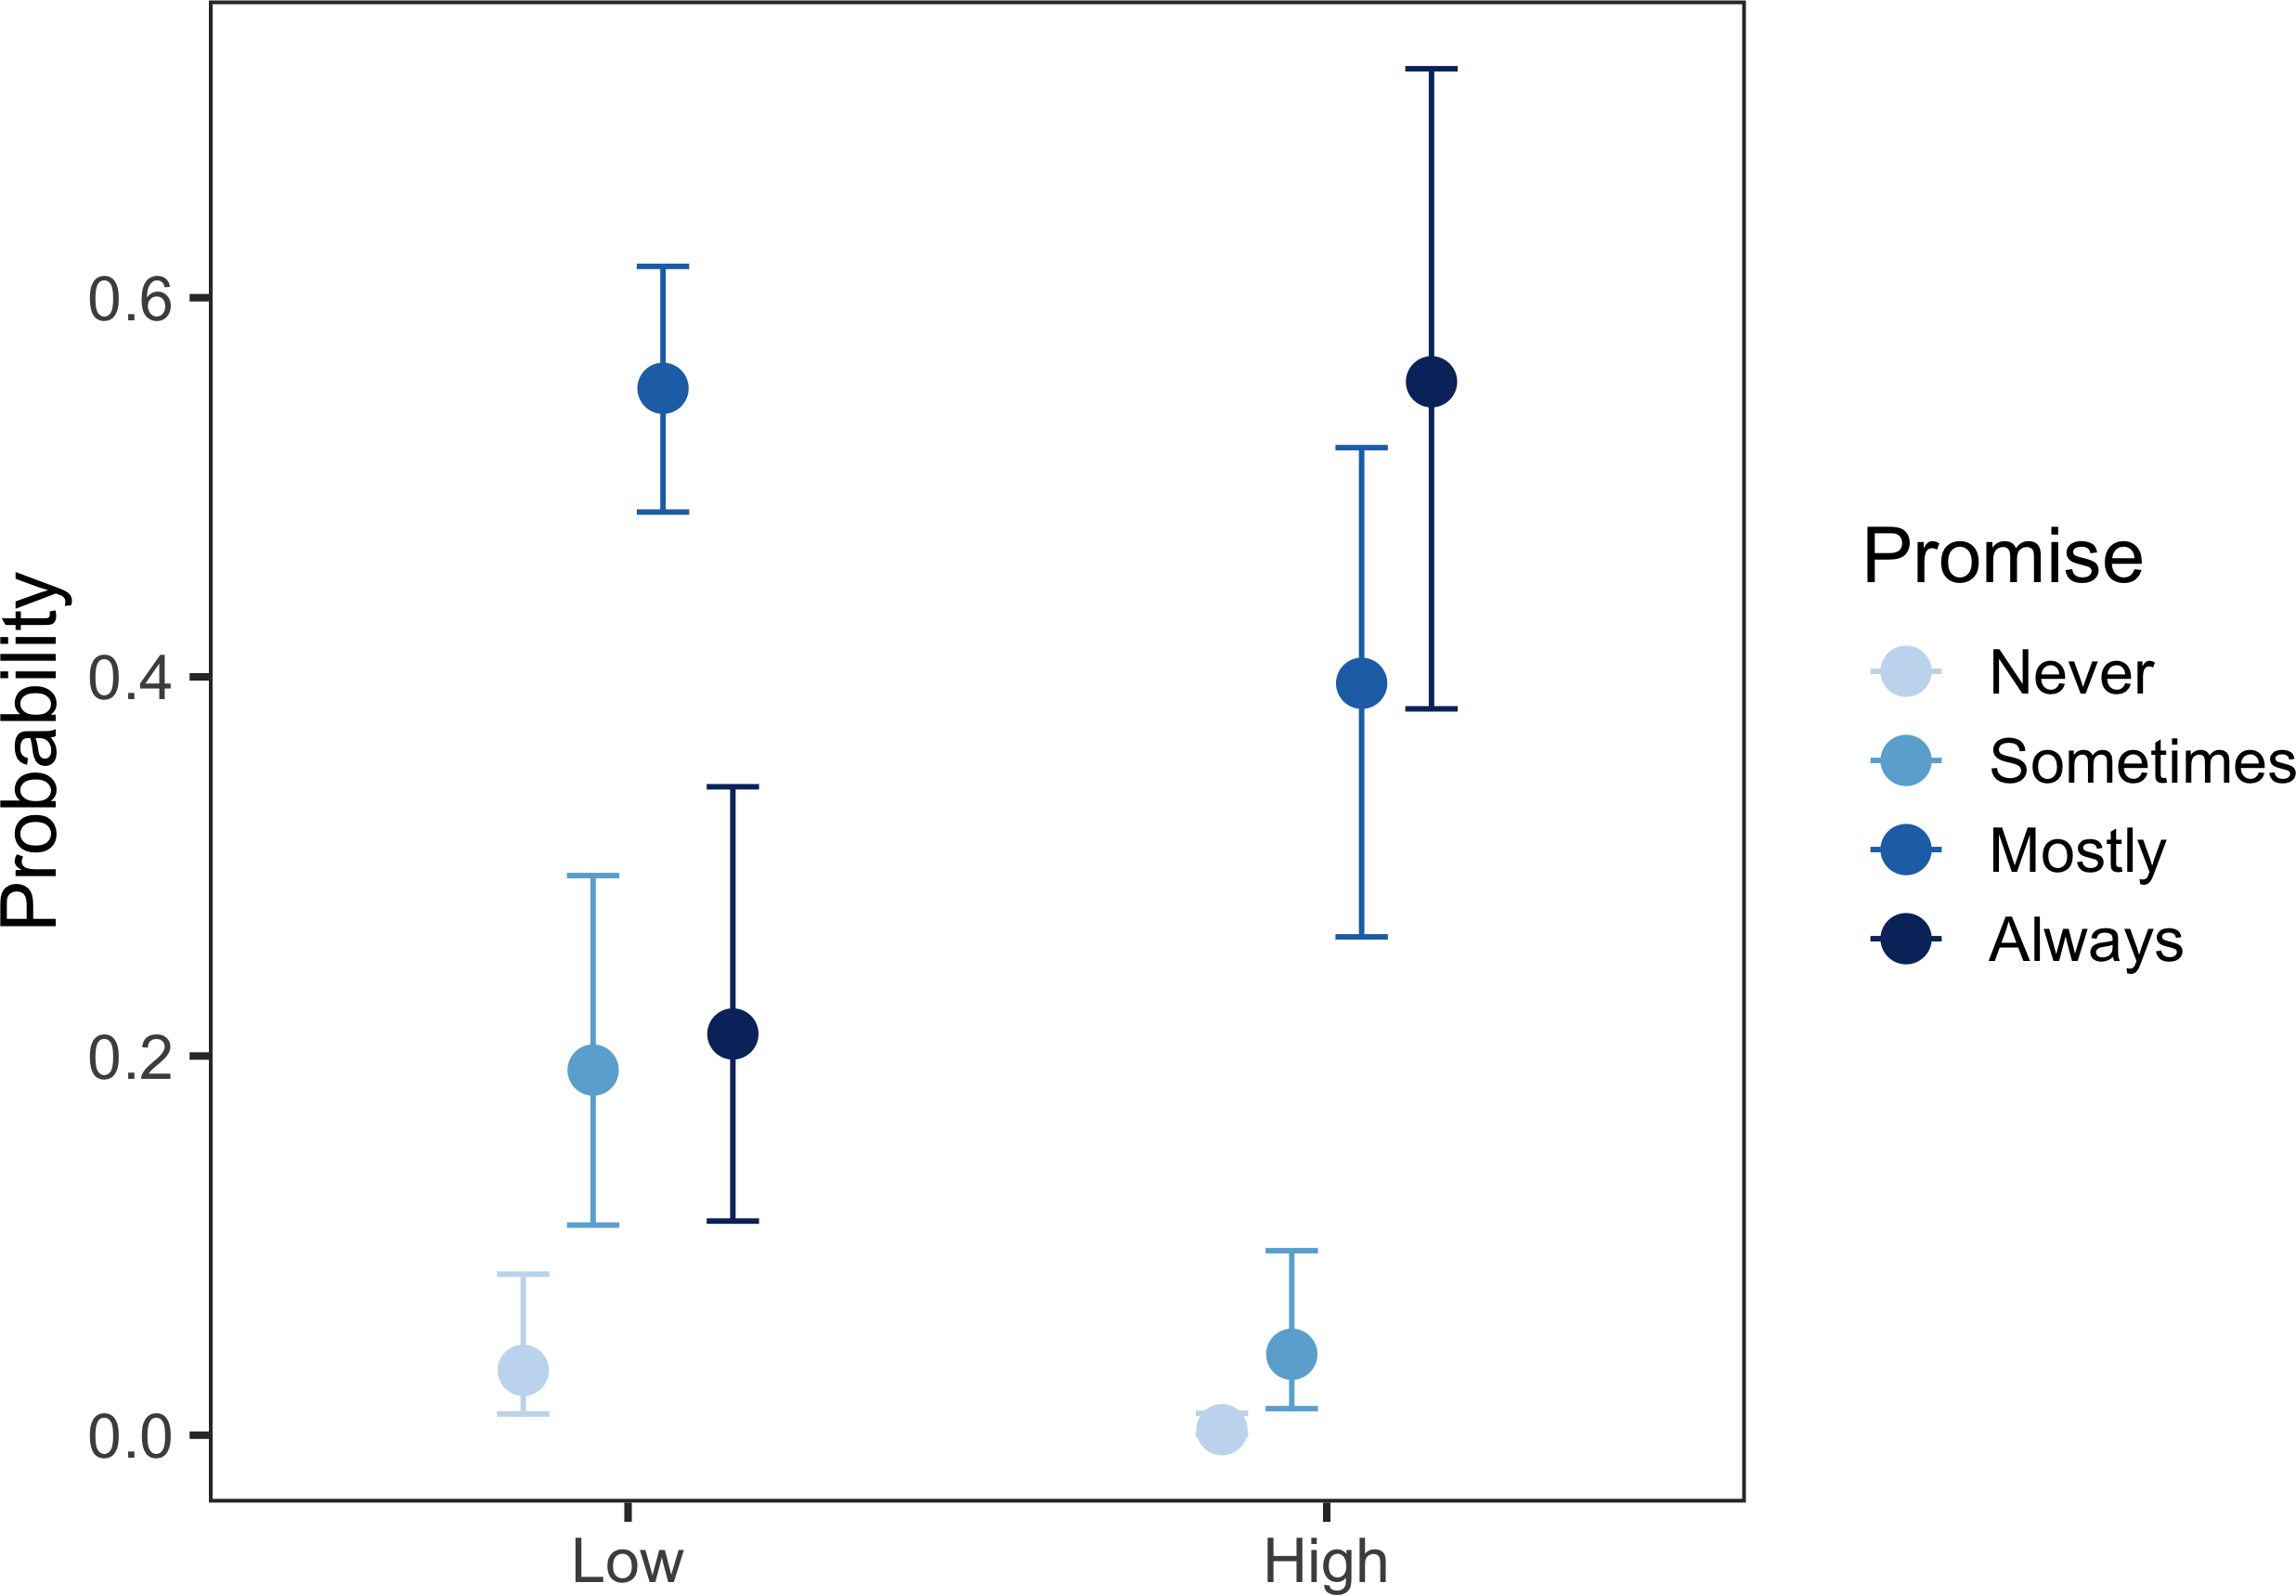
\includegraphics[width=0.8\linewidth]{behavioral-promises_files/figure-latex/fig7-1} 

}

\caption{Promise choices by group}\label{fig:fig7}
\end{figure}

\hypertarget{discussion}{%
\section{Discussion}\label{discussion}}

The goal of this study was to evaluate the effect of social closeness on
keeping and breaking promises, as well as on cooperation in a trust
game. Our results give evidence that zero social closeness increases the
probability of breaking the promise and it decreases monotonically as
social closeness increases. Likewise, as social closeness increases, so
does cooperation; high social closeness has an effect on decisions that
surpasses even those that all other experimental conditions. The most
interesting finding was that when subjects expressed high commitment to
cooperate (through choosing that they would always pay back), the
probability that they comply is also quite high. However, there is a
small but consistent proportion of transgressions according to our
inferences.

To our knowledge, this is the first experimental study that incorporates
social closeness as a predictor of the decision to break promises with
socially relevant partners. In previous studies, the participants remain
anonymous during the course of the tasks (Baumgartner et al. 2009),
their measurements to evaluate transgressions are self-reported (DePaulo
and Kashy 1998; DePaulo et al. 2004), they do not directly quantify the
breaking of promises (Vanberg 2008; Charness and Dufwenberg 2006), or as
we will discuss later, they use heterogeneous measures of social
closeness (Glaeser et al. 2000). Our experiment is the first one to
include a partner without social closeness (computer). Our data suggest
that the mere fact of considering that subjects play with a human
diminishes the probability of breaking the promise. It is more likely to
break the promise to the computer than to the stranger, even though that
partner was not known. Also, null social closeness is important because
it allows us to explore the intrinsic motivation to keep the promises.
If humans keep their word because it is morally correct, we would
anticipate that the probability of breaking a promise was very low in
the three partners and, particularly, the inference regarding the
probability of breaking the promise to the computer would include zero.
However, we found that, although low, the probability was greater than
zero, which provides evidence that seems to contradict, at least in
degree, the hypothesis of intrinsic motivation. We cannot exclude the
possibility that the subjects keep promises mainly due to moral
motivation because, even in the case of the computer, the subjects kept
a large proportion. We can, however, exclude that this is their only
motivation.

On the other hand, high social closeness allows us to explore the
instrumental motivation to keep promises (Baumgartner et al. 2009). In
our study, it was more likely to break the promise to the stranger than
to the friend. If humans keep their word to facilitate cooperation in
the future, we would anticipate that with a partner of high social
closeness (with whom they are very likely to cooperate, even after the
experiment) there would be less of a chance to break the promise. In
fact, the promise to friends was not broken on any occasion, hence the
inference in this case, was met.

The findings concerning motivations could be explained by the social
norm called ``conditional cooperation'', which indicates that the belief
that other people cooperate at high levels also induces high levels of
cooperation (Fehr and Schurtenberger 2018). Thus, the lack of certainty
regarding the decisions that the computer would make could explain the
probability of breaking the promise that exists towards this partner.
Similarly, the information that the subjects have regarding as their
friend's behavior -even before the experiment- could explain the high
levels of cooperation and keeping of promises towards this partner.

Cooperation has been studied with diverse experimental manipulations. In
one study, the contribution in a public goods game was evaluated during
several trials in a group made up of the same individuals (partners),
and compared to another group of new different subjects for each trial
(strangers) (Croson 1996). In the condition of partners the cooperation
was greater because it is a stable group compared to the group of
strangers. The mentioned study does not give details regarding the
recruitment of participants, so we could assume that even in the
condition of partners these are individuals who do not consider
themselves socially close.

Another study showed an increase in cooperation in a trust game when
individuals were socially close (Glaeser et al. 2000). In this study,
subjects knew each other and the researchers carefully measured several
variables regarding their social connection.However, some individuals
who arrived together were allowed to perform the task between themselves
and others were paired with unclear criteria. The above allows social
closeness between partners to be heterogeneous, allows for romantic
relationships and assumes that two individuals who come together to
class are considered close to each other. Also, since it is a study of
one-shot, it excludes the possibility of evaluating how the same subject
varies his behavior based on different levels of social closeness.

To try to homogenize social closeness between our subjects and their
partners, they performed the task with a same-sex friend considered to
be close, emphasizing their companion could not be a romantic or sexual
partner. Bayesian analysis of the IOS scale showed evidence in favor
that the degree of social closeness between 30 of our 45 subjects and
their friends was the same. Results of the two mentioned studies also
found that social closeness enhance cooperation (Croson 1996; Glaeser et
al. 2000), in the future would be valuable to homogenize both the
performed tasks and the statistical procedure used, to establish
similarity in effects magnitudes.

Our methodological contribution to the field is the use of Bayesian
inference tools: Hierarchical Models and Cumulative Models. The
Hierarchical Models, allowed us to model the effect of the experimental
conditions on the individual response. These models assume that lower
level observations (e.g.~decisions of each individual) are nested in
higher level units (e.g.~individual subjects). Within-subjects designs
have traditionally been analyzed with repeated measures AN(C)OVA,
however, Hierarchical Models grant the advantages of naturally dealing
with unbalanced data, include categorical and/or numerical predictors,
explicitly incorporate individual variability, among others (Vuorre and
Bolger 2018; Gelman and Hill 2006; McElreath 2018; Bürkner 2017).

In our case, the Hierarchical Model allowed us to capture how the
experimental conditions affected the decisions of each subject and the
differences between them. For example, there are obviously motivated
instrumental subjects such as number 8 or 12 who are very sensitive to
the identity of their investors and modify their cooperation under
social closeness. At the same time, there were notably intrinsic
subjects such as 9 and 10 who cooperate all the time regardless of who
their partners are. The Hierarchical Model naturally includes this
information for the estimation of population effects, which, if not
considered, would lead to inaccurate inferences(Bürkner 2017; Gelman and
Hill 2006; McElreath 2018).

On the other hand, the Cumulative Model allowed us to capture the
strength of the commitment expressed through promises. A very frequent
problem that has been pointed out recently is that analyzing ordinal
data with methods that assume that observations are metric can lead to
serious inference errors (Liddell and Kruschke 2018). The Cumulative
Models assumes that the observed responses come from the categorization
of a continuous latent variable (Bürkner and Vuorre 2019). In our study,
we could identify that groups with different payment proportions, which
in other studies have been called ``dishonest'' and
``honest''(Baumgartner et al. 2009; Baumgartner, Gianotti, and Knoch
2013), differ in the commitment they express through their promises.
Considering that the tools to perform the Cumulative Models are
relatively recent, in future studies, it would be valuable to also use
the new alternatives for inference.

Although the Hierarchical and Cumulative models are not tools
exclusively for Bayesian inference, their application from this approach
represents several advantages compared to frequentist statistics.
Classic problems such as multiple comparisons, the decision of when to
stop collecting subjects (stopping rule), or use of planned comparisons
versus post hoc, are not factors that affect the Bayesian approach
(Dienes 2011). In Bayesian inference, hypothesis testing makes formal
use of probability to express the plausibility of theories, and in our
case, we were able to obtain evidence ratios regarding the extent of our
data support hypotheses, regardless if these were proposed \emph{a
priori} or \emph{post hoc}.

\hypertarget{limitations}{%
\subsection{Limitations}\label{limitations}}

A limitation of this paper is the use of hypothetical rewards compared
to real rewards. A relatively recent study on decision-making reported
that there is more loss aversion when subjects have real monetary
rewards compared to hypothetical in a risk task (Xu et al. 2016).
However, other works do not report differences between the use of both
types of rewards in self-control, temporal and social discount tasks
(Locey, Jones, and Rachlin 2011; Johnson and Bickel 2006; Rachlin and
Jones 2006). Likewise, it can be argued that our results have
theoretical congruence (Fehr and Schurtenberger 2018) and are in the
same direction as other works that use real money (Croson 1996; Glaeser
et al. 2000), thus, there are not many reasons to expect that other
types of rewards would modify our results. Another possible limitation
is the use of multiple trials with each partner. Although the decision
to use repeated measures during our design serves more the purpose of
reducing contaminant sources and increasing internal validity (Maxwell,
Delaney, and Ken 2018), to have more clarity regarding the difference in
the intrinsic and instrumental motivations, the studies could benefit
from only include one trial for each partner. Play a one-shot with each
partner avoids the possibility that multiple trials could generate the
belief that the computer can also vary its behavior according to the
decisions of the trustee. Finally, subjects that performed the study
inside the MRI scanner may differ in their responses than subjects
outside of the scanner. However, our analysis did not show this
explicitly.

\hypertarget{conclusions}{%
\section{Conclusions}\label{conclusions}}

Subjects seem to keep their promises by a combination of
\emph{intrinsic} and \emph{instrumental} motivations. They are
predominantly ``nice people'' because they keep their word even with
investors with no social closeness. However, their trustworthiness is
far from perfect, since there is a small proportion of betrayals
committed towards this partner. It seems that if subjects cannot be sure
their investor will be a ``potential cooperator'', dishonesty may emerge
in the form of broken promises. Framing the finding in terms of the
theoretical predictions of the social norm ``conditional cooperation'',
social closeness decreases the probability of breaking the promise and
increases cooperation, and suggests the correspondence between
commitment expressed through promises and subsequent behavior.

\hypertarget{bibliography}{%
\section*{Bibliography}\label{bibliography}}
\addcontentsline{toc}{section}{Bibliography}

\hypertarget{refs}{}
\leavevmode\hypertarget{ref-Anderson2002}{}%
Anderson, D. Eric, Bella M. DePaulo, and Matthew E. Ansfield. 2002.
``The development of deception detection skill: A longitudinal study of
same-sex friends.'' \emph{Personality and Social Psychology Bulletin} 28
(4): 536--45. \url{https://doi.org/10.1177/0146167202287010}.

\leavevmode\hypertarget{ref-Aron1997}{}%
Aron, Arthur, Edward Melinat, Elaine N. Aron, Robert Darrin Vallone, and
Renee J. Bator. 1997. ``The experimental generation of interpersonal
closeness: A procedure and some preliminary findings.''
\emph{Personality and Social Psychology Bulletin} 23 (4): 363--77.
\url{https://doi.org/10.1177/0146167297234003}.

\leavevmode\hypertarget{ref-Balliet2010}{}%
Balliet, Daniel. 2010. ``Communication and cooperation in social
dilemmas: A meta-analytic review.'' \emph{Journal of Conflict
Resolution} 54 (1): 39--57.
\url{https://doi.org/10.1177/0022002709352443}.

\leavevmode\hypertarget{ref-Baumgartner2009}{}%
Baumgartner, Thomas, Urs Fischbacher, Anja Feierabend, Kai Lutz, and
Ernst Fehr. 2009. ``The Neural Circuitry of a Broken Promise.''
\emph{Neuron} 64 (5). Elsevier Ltd: 756--70.
\url{https://doi.org/10.1016/j.neuron.2009.11.017}.

\leavevmode\hypertarget{ref-Baumgartner2013}{}%
Baumgartner, Thomas, Lorena R R Gianotti, and Daria Knoch. 2013. ``Who
is honest and why: Baseline activation in anterior insula predicts
inter-individual differences in deceptive behavior.'' \emph{Biological
Psychology} 94 (1). Elsevier B.V.: 192--97.
\url{https://doi.org/10.1016/j.biopsycho.2013.05.018}.

\leavevmode\hypertarget{ref-Burkner2017}{}%
Bürkner, Paul-Christian. 2017. ``brms : An R Package for Bayesian
Multilevel Models Using Stan.'' \emph{Journal of Statistical Software}
80 (1). \url{https://doi.org/10.18637/jss.v080.i01}.

\leavevmode\hypertarget{ref-Burkner2019}{}%
Bürkner, Paul-Christian, and Matti Vuorre. 2019. ``Ordinal Regression
Models in Psychology: A Tutorial.'' \emph{Advances in Methods and
Practices in Psychological Science} 2 (1): 77--101.
\url{https://doi.org/10.1177/2515245918823199}.

\leavevmode\hypertarget{ref-Charness2006}{}%
Charness, Gary, and Martin Dufwenberg. 2006. ``Promises and
partnership.'' \emph{Econometrica} 74 (6): 1579--1601.
\url{https://doi.org/10.1111/j.1468-0262.2006.00719.x}.

\leavevmode\hypertarget{ref-Croson1996}{}%
Croson, Rachel T.A. 1996. ``Partners and strangers revisited.''
\emph{Economics Letters} 53 (1): 25--32.
\url{https://doi.org/10.1016/S0165-1765(97)82136-2}.

\leavevmode\hypertarget{ref-DePaulo2004}{}%
DePaulo, Bella M, Matthew E Ansfield, Susan E Kirkendol, and Joseph M
Boden. 2004. ``Serious Lies.'' \emph{Basic \& Applied Social Psychology}
26 (2/3): 147--67. \url{https://doi.org/10.1207/s15324834basp2602\&3_4}.

\leavevmode\hypertarget{ref-DePaulo1998}{}%
DePaulo, Bella M., and Deborah A. Kashy. 1998. ``Everyday Lies in Close
and Casual Relationships.'' \emph{Journal of Personality and Social
Psychology} 74 (1): 63--79.
\url{https://doi.org/10.1037/0022-3514.74.1.63}.

\leavevmode\hypertarget{ref-Dienes2011}{}%
Dienes, Zoltan. 2011. ``Bayesian versus orthodox statistics: Which side
are you on?'' \emph{Perspectives on Psychological Science} 6 (3):
274--90. \url{https://doi.org/10.1177/1745691611406920}.

\leavevmode\hypertarget{ref-Fareri2014}{}%
Fareri, Dominic S., and Mauricio R. Delgado. 2014. ``Differential reward
responses during competition against in- and out-of-network others.''
\emph{Social Cognitive and Affective Neuroscience} 9 (4): 412--20.
\url{https://doi.org/10.1093/scan/nst006}.

\leavevmode\hypertarget{ref-Fehr2003}{}%
Fehr, Ernst, and Urs Fischbacher. 2003. ``The nature of human
altruism.'' \emph{Nature} 425 (6960). Nature Publishing Group: 785--91.
\url{https://doi.org/10.1038/nature02043}.

\leavevmode\hypertarget{ref-Fehr2018}{}%
Fehr, Ernst, and Ivo Schurtenberger. 2018. ``Normative foundations of
human cooperation review-article.'' \emph{Nature Human Behaviour} 2 (7).
Springer US: 458--68. \url{https://doi.org/10.1038/s41562-018-0385-5}.

\leavevmode\hypertarget{ref-Fischbacher2013a}{}%
Fischbacher, Urs, and Franziska Föllmi-Heusi. 2013. ``Lies in
disguise-an experimental study on cheating.'' \emph{Journal of the
European Economic Association} 11 (3): 525--47.
\url{https://doi.org/10.1111/jeea.12014}.

\leavevmode\hypertarget{ref-Gelman2006}{}%
Gelman, Andrew, and Jennifer Hill. 2006. \emph{Data analysis using
regression and multilevel/hierarchical models.}
\url{https://doi.org/10.2277/0521867061}.

\leavevmode\hypertarget{ref-Glaeser2000}{}%
Glaeser, Edward, David Laibson, Jose Sceinkman, and Christine Soutter.
2000. ``Measuring Trust.'' \emph{The Quartely Journal of Economics} 115
(3): 811--46.

\leavevmode\hypertarget{ref-Gneezy2005}{}%
Gneezy, Uri. 2005. ``Deception: The role of consequences.''
\emph{American Economic Review} 95 (1): 384--94.
\url{https://doi.org/10.1257/0002828053828662}.

\leavevmode\hypertarget{ref-Gneezy2013}{}%
Gneezy, Uri, Bettina Rockenbach, and Marta Serra-Garcia. 2013.
``Measuring lying aversion.'' \emph{Journal of Economic Behavior and
Organization} 93. Elsevier B.V.: 293--300.
\url{https://doi.org/10.1016/j.jebo.2013.03.025}.

\leavevmode\hypertarget{ref-Holt-Lunstad2018}{}%
Holt-Lunstad, Julianne. 2018. ``Why Social Relationships are Important
for Physical Health: A Systems Approach to Understanding and Modifying
Risk and Protection.'' \emph{Ssrn}, no. October 2017: 1--22.
\url{https://doi.org/10.1146/annurev-psych-122216-011902}.

\leavevmode\hypertarget{ref-Johnson2006}{}%
Johnson, Matthew W, and Warren K Bickel. 2006. ``Within-subject
comparison of real and hypothetical money rewards in delay
discounting.'' \emph{Journal of the Experimental Analysis of Behavior}
77 (2): 129--46. \url{https://doi.org/10.1901/jeab.2002.77-129}.

\leavevmode\hypertarget{ref-Lee2014}{}%
Lee, Michael D., and Eric-Jan Wagenmakers. 2014. \emph{Bayesian
Cognitive Modeling}. \url{https://doi.org/10.1017/cbo9781139087759}.

\leavevmode\hypertarget{ref-Liddell2018}{}%
Liddell, Torrin M., and John K. Kruschke. 2018. ``Analyzing ordinal data
with metric models: What could possibly go wrong?'' \emph{Journal of
Experimental Social Psychology} 79 (November 2017). Elsevier: 328--48.
\url{https://doi.org/10.1016/j.jesp.2018.08.009}.

\leavevmode\hypertarget{ref-Locey2011}{}%
Locey, Matthew L, Bryan A Jones, and Howard Rachlin. 2011. ``Real and
hypothetical rewards in self-control and social discounting.''
\emph{Judgment and Decision Making} 6 (6): 552--64.

\leavevmode\hypertarget{ref-Maxwell2018}{}%
Maxwell, Scott E., Harold D. Delaney, and Kelley Ken. 2018.
\emph{Designing experiments and analyzing data: a model comparison
perspective}. 3rd edition. New York: Routledge.

\leavevmode\hypertarget{ref-Mazar2008}{}%
Mazar, Nina, On Amir, and Dan Ariely. 2008. ``The Dishonesty of Honest
People: A Theory of Self-Concept Maintenance.'' \emph{Journal of
Marketing Research} 45 (6): 633--44.
\url{https://doi.org/10.1509/jmkr.45.6.633}.

\leavevmode\hypertarget{ref-McElreath2018}{}%
McElreath, Richard. 2018. \emph{Statistical rethinking: A bayesian
course with examples in R and stan}.
\url{https://doi.org/10.1201/9781315372495}.

\leavevmode\hypertarget{ref-Peirce2019}{}%
Peirce, Jonathan, Jeremy R. Gray, Sol Simpson, Michael MacAskill,
Richard Höchenberger, Hiroyuki Sogo, Erik Kastman, and Jonas Kristoffer
Lindeløv. 2019. ``PsychoPy2: Experiments in behavior made easy.''
\emph{Behavior Research Methods} 51 (1): 195--203.
\url{https://doi.org/10.3758/s13428-018-01193-y}.

\leavevmode\hypertarget{ref-Peirce2008}{}%
Peirce, Jonathan W. 2008. ``Generating stimuli for neuroscience using
PsychoPy.'' \emph{Frontiers in Neuroinformatics} 2.
\url{https://doi.org/10.3389/neuro.11.010.2008}.

\leavevmode\hypertarget{ref-Rachlin2006}{}%
Rachlin, Howard, and Bryan Jones. 2006. ``Social Discounting.''
\emph{Psychological Science} 17 (4): 283--86.

\leavevmode\hypertarget{ref-R2019}{}%
R Core Team. 2019. \emph{R: A Language and Environment for Statistical
Computing}. Vienna, Austria: R Foundation for Statistical Computing.
\url{https://www.R-project.org/}.

\leavevmode\hypertarget{ref-Schad2019}{}%
Schad, Daniel, Michael Betancourt, and Shravan Vasishth. 2019. ``Toward
a principled Bayesian workflow in cognitive science.''
\url{osf.io/b2vx9}.

\leavevmode\hypertarget{ref-Sip2015}{}%
Sip, Kamila E., David V. Smith, Anthony J. Porcelli, Kohitij Kar, and
Mauricio R. Delgado. 2015. ``Social closeness and feedback modulate
susceptibility to the framing effect.'' \emph{Social Neuroscience} 10
(1): 35--45. \url{https://doi.org/10.1080/17470919.2014.944316}.

\leavevmode\hypertarget{ref-GSS2018}{}%
Smith, Tom, Michael Davern, Jeremy Freese, and Michael Hout. 2018. ``GSS
Data Explorer \textbar{} NORC at the University of Chicago.''
\url{https://gssdataexplorer.norc.org/variables/5067/vshow}.

\leavevmode\hypertarget{ref-Rstan2018}{}%
Stan Development Team. 2018. ``RStan: The R Interface to Stan.''
\url{http://mc-stan.org/}.

\leavevmode\hypertarget{ref-Tough2017}{}%
Tough, Hannah, Johannes Siegrist, and Christine Fekete. 2017. ``Social
relationships, mental health and wellbeing in physical disability: A
systematic review.'' \emph{BMC Public Health} 17 (1). BMC Public Health:
1--18. \url{https://doi.org/10.1186/s12889-017-4308-6}.

\leavevmode\hypertarget{ref-UN2018}{}%
UN. 2018. ``Global Cost of Corruption at Least 5 Per Cent of World Gross
Domestic Product, Secretary-General Tells Security Council, Citing World
Economic Forum Data.''
\url{https://www.un.org/press/en/2018/sc13493.doc.htm}.

\leavevmode\hypertarget{ref-Vanberg2008}{}%
Vanberg, Christoph. 2008. ``Why Do People Keep Their Promises? An
Experimental Test of Two Explanations1.'' \emph{Econometrica} 76 (6):
1467--80. \url{https://doi.org/10.3982/ECTA7673}.

\leavevmode\hypertarget{ref-Vuorre2018}{}%
Vuorre, Matti, and Niall Bolger. 2018. ``Within-subject mediation
analysis for experimental data in cognitive psychology and
neuroscience.'' \emph{Behavior Research Methods} 50 (5): 2125--43.
\url{https://doi.org/10.3758/s13428-017-0980-9}.

\leavevmode\hypertarget{ref-Xu2016}{}%
Xu, Sihua, Yu Pan, You Wang, Andrea M Spaeth, Zhe Qu, and Hengyi Rao.
2016. ``Real and hypothetical monetary rewards modulate risk taking in
the brain.'' \emph{Scientific Reports} 6.
\url{https://doi.org/10.1038/srep29520}.

\bibliographystyle{spbasic}
\bibliography{bibliography.bib}

\end{document}
